% PROGRAMA DE PÓS-GRADUAÇÃO EM ECONOMIA APLICADA
% UNIVERSIDADE FEDERAL DO RIO GRANDE - FURG

% ===========================================================

\documentclass[a4paper, 17pt]{extarticle}

%%%%%%%%%%%%%%%%%%%%%%%%% PACOTES %%%%%%%%%%%%%%%%%%%%%%%%%%%%%%%%%%
 
\usepackage[margin = 0.5in, bottom = 2in]{geometry}
\usepackage[utf8]{inputenc}
\usepackage[T1]{fontenc}
\usepackage{graphicx}
\usepackage{enumitem}
\usepackage{multicol}
\usepackage{subcaption}
\usepackage{arydshln}
%\usepackage{pdfcomment}
\usepackage{parskip}
\usepackage{xcolor}
\usepackage{lipsum}	
\usepackage{amsfonts,amsmath,amssymb, amsthm, pifont}
\usepackage{booktabs}
\usepackage[colorlinks=true, linkcolor=blue, citecolor=blue, urlcolor=blue]{hyperref} 
\usepackage{todonotes} 
\usepackage{dsfont}
\usepackage{cancel}
\usepackage{layout}
\usepackage[most]{tcolorbox}
\usepackage{tikz}
\usepackage{tikz-3dplot} 
\usepackage[absolute, overlay]{textpos} 
\usetikzlibrary{arrows.meta, cd, patterns, patterns.meta}
\usepackage[bottom]{footmisc}

% Configuração da Fonte
\usepackage{times} % Fonte: Times New Roman

% PACOTES ESSENCIAIS
\usepackage{caption}  
\usepackage{titlesec}  

\titleformat{\section}
  {\normalfont\Large\bfseries} % formato de la fuente
  {\S \hspace{-0cm} \thesection}              % etiqueta de la sección (con símbolo ♦)
  {0.5em}                        % espacio entre el número y el título
  {}                           % código antes del título

%\setlength{\footskip}{10pt} % Espacio entre texto y pie de página
\renewcommand{\footnoterule}{\vspace{5pt}\hrule width 0.3\linewidth\vspace{5pt}}
\setlength{\textheight}{750pt}
%\setlength{\textwidth}{530pt}
%\setlength{\headsep}{10pt}
%\setlength{\marginparwidth}{145pt}
%\setlength{\marginparsep}{12pt}
%\setlength{\topmargin}{-60pt}

\definecolor{verdeoscuro}{RGB}{0,100,0} % Un verde bastante oscuro
\definecolor{rojoscuro}{RGB}{139,0,0} % rojo oscuro tipo "DarkRed"

%\pagestyle{empty}

\newcommand{\ejemplo}[1]{%
  \begin{tcolorbox}[colframe=verdeoscuro, colback=white!1, boxrule=0.8pt]
    #1
  \end{tcolorbox}
}
\newcommand{\alerta}[1]{%
  \begin{tcolorbox}[colframe=red, colback=white!1, boxrule=0.8pt]
    #1
  \end{tcolorbox}
}
\newcommand{\demo}[1]{%
  \begin{tcolorbox}[colframe=gray, colback=white!1, boxrule=0.8pt]
    \textcolor{gray}{#1}
  \end{tcolorbox}
}

\todostyle{orange}{
    linecolor=orange,        % Flecha negra
    bordercolor=orange,      % Borde negro
    textcolor=black!90,      % Borde negro
    backgroundcolor=white!33,  % Sin relleno de color
    size=\scriptsize           % Tamaño de texto
}
\todostyle{green}{
    linecolor=verdeoscuro,        % Flecha negra
    bordercolor=verdeoscuro,      % Borde negro
    textcolor=black!90,      % Borde negro
    backgroundcolor=white!33,  % Sin relleno de color
    size=\scriptsize           % Tamaño de texto
}
\todostyle{red}{
    linecolor=red,        % Flecha negra
    bordercolor=red,      % Borde negro
    textcolor=black!90,      % Borde negro
    backgroundcolor=white!33,  % Sin relleno de color
    size=\scriptsize           % Tamaño de texto
}
\todostyle{red2}{
  linecolor=rojoscuro,        % Flecha negra
  bordercolor=rojoscuro,      % Borde negro
  textcolor=black!90,      % Borde negro
  backgroundcolor=white!33,  % Sin relleno de color
  size=\scriptsize           % Tamaño de texto
}
\todostyle{gris}{
  linecolor=gray,        % Flecha negra
  bordercolor=gray,      % Borde negro
  textcolor=black!90,      % Borde negro
  backgroundcolor=white!33,  % Sin relleno de color
  size=\scriptsize           % Tamaño de texto
}
\begin{document} %Início do Documento

%\layout
%\newpage 


%%%%%%%%%%%%%%%%%%%%%%%%%  MEU PREAMBULO %%%%%%%%%%%%%%%%%%%%%%%%%%%%%%%%%

\makeatletter
\renewcommand\@makefnmark{%
  \hbox{\@textsuperscript{\color{magenta}\normalfont\@thefnmark}}}
\renewcommand\@makefntext[1]{%
  \noindent\makebox[1.8em][r]{\textsuperscript{\color{magenta}\@thefnmark}}#1}
\makeatother

\theoremstyle{definition}
\newtheorem*{definition}{\rotatebox{45}{\large \(\square\)}}

\theoremstyle{plain}
\newtheorem*{lemma}{{\scriptsize \(\square\)}}
\newtheorem*{proposition}{{\large \(\square\)}}
\newtheorem*{theorem}{{\large \(\blacksquare\)}} 

\makeatletter
% Eliminar la puntuación del estilo 'plain' y 'definition'
\def\@thm@headpunct{} % Elimina el punto de los títulos de los teoremas

% Modificar el estilo de 'plain' y 'definition'
\def\th@plain{%
  %\thm@headfont{\normalfont\bfseries} % Mantener la fuente normal, sin negrita
  %\thm@notefont{\normalfont} % El texto de la nota (si la hay) no será en negrita
  \thm@headpunct{} % Sin puntuación adicional 
}

\def\th@definition{%
  %\thm@headfont{\normalfont\bfseries} % Fuente normal para el título
  %\thm@notefont{\normalfont} % El texto de la nota (si la hay) no será en negrita
  \thm@headpunct{} % Sin puntuación adicional
}

\def\th@remark{%
  %\thm@headfont{\normalfont\bfseries} % Fuente normal para el título
  %\thm@notefont{\normalfont} % El texto de la nota (si la hay) no será en negrita
  \thm@headpunct{} % Sin puntuación adicional
}
\makeatother



\theoremstyle{remark}
\newtheorem*{example}{\textcolor{verdeoscuro}{\underline{{Exemplo}}}}
\newtheorem*{exercise}{\textcolor{rojoscuro}{\underline{{Exercise}}}}\theoremstyle{remark}
\newtheorem*{note}{\textnormal{\emph{Nota. }}}
\newtheorem*{corollary}{\textnormal{\emph{Corolário. }}}

\newcommand{\id}{\mathds{1}}
\newcommand{\R}{\mathbb{R}}
\newcommand{\B}{\mathbb{B}}
\newcommand{\Ei}{}
\newcommand{\Ef}{}
\newcommand{\N}{\mathbb{N}}
\newcommand{\U}{\mathcal{U}}
\newcommand{\V}{\mathcal{V}}
\newcommand{\E}{\mathbb{S}}
\newcommand{\ab}{^{\text{\ding{71}}}}
\newcommand{\ce}{^{\text{\ding{70}}}}
\newcommand{\x}{\textbf{x}}
\newcommand{\y}{\textbf{y}}


\setlength{\columnsep}{1in}

%\begin{multicols}{2}

\-\vspace{-1.3cm} 

\par\noindent \includegraphics[width = \linewidth]{Imagens/Header.png} 

%%%%%%%%%%%%%%%%%%%%%%%% CONFIG. DO TÍTULO %%%%%%%%%%%%%%%%%%%%%%%%

\begin{center} %Inicia a centralização
{%{ \Large QUALI SURVIVAL GUIDE COLLECTION} \\ 
 \LARGE \textbf{\(^{+1}\)Notas de Análise no \(\mathbb{R}^n\)}} \vspace{0.1in}   \\
 { \today }\\ 
 {\small
 \vspace{0.4cm}\emph{"Tudo posso naquele que me fortalece" }\hfill Nestor Heli Aponte Avila\(^{1}\) \\ 
  
Elon 4:13 \hfill \href{mailto:n267452@dac.unicamp.br}{\url{n267452@dac.unicamp.br}}} %\\
%Prof. Piper Pimienta \\
%\href{mailto:pipe@dac.unicamp.br}{\url{pipe@dac.unicamp.br}}}
\end{center} %Finaliza a centralização
\- \vspace{-1cm}

{\small ** Conteúdo basado na disciplina MM720 (Análise no R(n)) ministrada pelo professor Tiago Jardím Fonseca no período 2025-I. **\vspace{0.3cm}}%, destinado àqueles que já possuem alguma familiaridade com o assunto, pois não contém demonstrações formais, apenas as ideias por trás delas. Sinceramente, um fã da simplicidade. \\ 


%%%%%%%%%%%%%%%%%%%%%%%%% CONTENIDO %%%%%%%%%%%%%%%%%%%%%%%%%%%%%%%%%%
{\large \textbf{Notação}} \hfill \text{\rotatebox{45}{\large $\square$}}  Definição \hfill \((-)^{\text{\ding{71}}}\)  Aberto \hfill  \((-)^{\text{\ding{70}}}\) Fechado \\ 
\- \hspace{4.7cm}{\scriptsize$\square$} \ Lema \hspace{2.9cm} {\large$\square$} \ Proposição \hspace{1.3cm}  {\large $\blacksquare$}  \ Teorema
%\begin{center}
%  \setlength{\tabcolsep}{20pt}
%  \begin{tabular}{c c c }
%     \vspace{0.05in}  & &\\ 
%      &   
%  \end{tabular}
%\end{center}

\section{Derivadas Direcionais}

\begin{definition}%[\textbf{Derivada Direccional}] 
  Seja \(f:U\ab\subseteq \R^n\to \mathbb{R}\) uma função escalar. Para \(\vec{v}\in \mathbb{R}^n\) e \(p\in U\), a $v$-\textit{direcional derivada} de \(f\) em \(p\), se existir, é dada por 
  {\begin{equation*}
  \frac{\partial f}{\partial v}(p) := \lim\limits_{h\to 0} \frac{f(p+hv) - f(p)}{h} \hspace{0in} \sim \hspace{0in} f(p+hv) = f(p) + \frac{\partial f }{\partial v}(p)\cdot h + \sigma(h).
  \end{equation*}}
  \begin{note}
  Se \(v = e_i\) então \(\frac{\partial f}{\partial x_i}(p)\) é a $i$-ésima \textit{derivada parcial} de $f$ em $p$.
  \end{note}
\end{definition}

\Ei
\ejemplo{ \centering \(\exists \alpha \in \R : f(p+hv) = f(p) + \alpha h + \sigma(h)\Rightarrow \frac{\partial f }{\partial v}(p) = \alpha\)
\tcblower
\begin{example}
  \(f:\R^2 \ni \x \mapsto \|\x \|^2\in \R \). \textcolor{gray}{\(\rightarrow \) Use produto interno e encontre \(\alpha\)} %\todo[green]{Calculate the limit, develop with intern product properties and find \(\alpha\).}.
\end{example}}
%\begin{exercise}
%  Let \(\lambda\in \R\) and \(\vec{v},\vec{\omega} \in \R^n\). Show that \(\frac{\partial f }{\partial \lambda v} (p) = \lambda \frac{\partial f }{\partial v}(p)\). Does the following equality always hold? \(\frac{\partial f }{\partial (v+\omega)}(p) = \frac{\partial f }{\partial v}(p) + \frac{\partial f }{\partial \omega}(p )\). \textcolor{gray}{\(\rightarrow\) Manipulate and restate the expresion of the limit} 
%\end{exercise}
%\begin{example}
%  \(g :\R^2\backslash\{0\}\to \R\) such that \((x,y) \mapsto \arctan (y/x)\). \textcolor{gray}{\(\rightarrow\) Just calculate} 
%\end{example}
\alerta{ \centering
\(\forall j\leq n, \ \exists \frac{\partial f}{\partial x_j}(p)\) \textcolor{red}{\(\nRightarrow \)} \(\forall \vec{v} \in \R^n, \ \exists \frac{\partial f}{\partial v}(p)\) \textcolor{red}{\(\nRightarrow\)} \(f\) continua em \(p\)
\tcblower 
 \begin{example}{ 
   \( (x,y) \mapsto x+y, \text{ \ se }x=0\ \text{or}\ y=0\)}, nula no caso contrario. \textcolor{gray}{\(\rightarrow\) Prove diferentes direções em \(0\)}
\end{example}
%\- \tcblower
\begin{example}
  \(0\neq (x,y) \mapsto  \frac{xy^2}{\|x\|^2}\), nula em \(0\). \textcolor{gray}{\(\rightarrow\) Estude a continuidade no \(0\)}
\end{example}
}
 
\begin{definition}[\emph{Conexidade}]
\(X\ab\subseteq \R^n\) é \emph{conexo} sse \(\nexists  U\ab,V\ab\subseteq \R^n\) não vazios tais que \(U\cap V \neq \emptyset\) e \(X \subseteq U\cup V\). 
\end{definition}

\Ei

\begin{lemma}
  Se \(U\ab\subseteq \R^n\) é conexo, então \(\forall p,q\in U, \exists \Gamma\) caminho poligonal em \(U\) com vértices \(p = p_0, p_1, \ldots, p_k = q,\) tais que \(p_{i+1}- p_i\) é colinear com algum \(e_j\). 
  \textcolor{gray}{\(\rightarrow \) É por construção, só lembre que \(U\) é aberto.}
  %\footnote{O lema só vale em \(U\) aberto, pense em \({\mathbb{S}^{1}}\).}
\end{lemma}

%\- \vspace{-0.3cm}\\ 
\begin{proposition}
  Seja \(U\ab\subseteq \R^n\) conexo e \(f:U\to \R\) função tal que \(\forall p \in U,\ \forall i\leq n\) as derivadas \(\frac{\partial f}{\partial x_i}(p) = 0\) em \(U\), então \(f\) é constante. 
\end{proposition}
\demo{Use o lemma, aplique TVM para \(\varphi(t) = f(p_i + te_j)\), quem é \(\varphi{'} (\theta)\)?}
%\begin{exercise}
%  If $\forall p\in U, \exists M>0$ such that \(\Big|\frac{\partial f}{\partial x_i}(p) \Big|\leq M\) then $f$ is continuous in \(U\). \textcolor{gray}{\(\rightarrow \) Re-express \(f(p+v)- f(p)\) and get summands to which to apply MVT (case \(\R\)) as we did in the previous proposition}
%\end{exercise}
\section{Funções de Classe \(C^k\)}
 
\begin{definition}
    Seja \(f: U\ab\subseteq \R^n \to \R\) tal que \(\forall p \in U, \exists \frac{\partial f }{\partial x_i}(p): U \to \R\), definimos a \emph{derivada de segundo ordem} de \(f\) como 
    \[\frac{\partial^2 f}{\partial x_j \partial x_i}(p) := \frac{\partial}{\partial x_j}\left(\frac{\partial f}{\partial x_i}\right)(p).\]
\end{definition}
\begin{note}
    O ordem é importante, em geral. De forma análoga, definimos as $k$-ésimas derivadas  de \(f\).
\end{note}

\begin{definition}
    Seja \(k\in \{0\}\cup \N \). Uma função \(f:U\ab\subseteq \R^n\to \R\) é de classe \(C^k(U)\) se \(\forall p \in U, \forall m \leq k, \exists \partial^m f(p)\) continua em \(p\). 
\end{definition}

\begin{note}
\(f \in C^0\Leftrightarrow f\) continua; \(f \in C^\infty \Leftrightarrow f\) é \emph{suave}.  
\end{note}
%Note que van a existir varias derivadas de orden \(k\), dependiendo del valor de \(n\)
\begin{example}
    O anel de polinômios \(\R[x_1,\ldots,x_n]\subseteq C^\infty(\R^n)\). 
\end{example}
\begin{example}
    \(\det(T): M_{n}(\R) \cong \R^{n^2}\to \R\) é de classe \(C^\infty\). \textcolor{gray}{\(\rightarrow\) É polinomial}
\end{example}
\begin{example}
    Seja \(f: x\mapsto x^{1/3}\), então \(f \in C^0(\R)\) mais não é de classe \(C^1\) em \(0\). \textcolor{gray}{\(\rightarrow\) Veja o que acontece com o límite nesse punto}
\end{example}

%\begin{textblock*}{5cm}(14.75cm, 1cm) % ancho de la caja y posición (x,y)
%  \includegraphics[width=5cm]{Imagens/2-1.pdf}
%\end{textblock*}
%\begin{textblock*}{5cm}(15.4cm, 1.3cm) % ancho de la caja y posición (x,y)
%  \scriptsize \textcolor{blue}{---} \ \(\sqrt[3]{t} \)
%\end{textblock*}
%    Muestre que \(C^k(U)\) es una \(\R\)-álgebra\todo[orange,noline]{\(f \in C^k(U) \Rightarrow\frac{1}{f}\in C^k(U) \) siempre que \(f(\textbf{x})\neq 0\) en \(U\)} conmutativa, con la suma y el produto usual de funciones. Además de es eso pruebe que 
%    \[C^0(U)\supsetneq C^1(U)\supsetneq \cdots \supsetneq C^\infty(U), \]
%    Y note que los elementos inversos son aquellos que no se anulan.  \textcolor{gray}{\(\rightarrow\) Ni idea}
%\end{exercise}
%\begin{example}
%    \(\displaystyle f(x,y) = \begin{cases}
%        \frac{xy(x^2+y^2)}{x^2+y^2}, \ &\text{si}\ (x,y)\neq 0 \\
%        0, \ &\text{e.o.c.}
%    \end{cases}\). \textcolor{gray}{\(\rightarrow\) Estudie diff en \(p=0\)}
%\end{example}


\begin{theorem}[\emph{Schwarz}] 
    Se \(f \in C^2(U)\), então \(\forall i,j \leq n\) temos  
    \[\frac{\partial^2 f}{\partial x_i \partial x_j} = \frac{\partial^2 f }{\partial x_j \partial x_i}.\]
\end{theorem}

\demo{\parbox[a]{0.25\linewidth}{\- }\parbox[b]{0.75\linewidth}{Basta ver \(n=2\). Defina \( S = f(x+h, y+k) - f(x+h,y) - f(x, y+k) + f(x,y)\) e \(\varphi(t) = f(t, y+k) - f(t, y)\), aplique TVM \(\times 2\) e manobre até obter uma igualdade a \(S\). O resultado segue de fazer o mesmo a \(\psi(t)\), fixando a outra coordenada.}}
\begin{tikzpicture}[scale = 0.8, >=to, shift={(2.1cm,3.6cm)}, baseline={(current bounding box.center)}, remember picture, overlay]

  % Círculo dashed
  \draw[dashed, color = gray, opacity = 0.7] (0.6,-1.8) arc[start angle = -60, end angle = 60, radius = 2.4cm];

  % Coordenadas del rectángulo
  \coordinate (A) at (-1,1.5);
  \fill[gray] (A)  circle (2pt);
  \coordinate (B) at (0.7,1.5);
  \fill[gray] (B)  circle (2pt);
  \coordinate (C) at (0.7,-0.8);
  \fill[gray] (C)  circle (2pt);
  \coordinate (D) at (-1,-0.8);
  \fill[gray] (D)  circle (2pt);

  % Dibujo del rectángulo
  \fill[color = gray, opacity = 0.3] (A) -- (B) -- (C) -- (D) -- cycle;
  \draw[thick, gray] (A) -- (B) -- (C) -- (D) -- cycle;

  % Etiquetas de los vértices
  \node[above, color = gray]  at (A) {\tiny$(x,y+k)$};
  \node[above right, color = gray] at (B) {\tiny$(x+h,y+k)$};
  \node[below right, color = gray] at (C) {\tiny$(x+h,y)$};
  \node[below, color = gray]  at (D) {\tiny$(x,y)$};

\end{tikzpicture}
\- \vspace{-1cm}
\begin{corollary}
    Se \(f\in C^k(U)\) então não importa o ordem em que são tomadas as derivadas de ordem \(m\leq k\). \textcolor{gray}{\(\rightarrow\) É uma questão de trabalhá-las 2 a 2}
\end{corollary} 
\section{O Diferencial} 

\begin{definition}
    Seja \(U\ab\subseteq \R^n\). Uma função \(f:U \to \R\) é \emph{diff} em \(p\in U \) sse \(\exists \ell : \R^n \to \R\) lineal, tal que 
    \[f(p+v) = f(p) + \ell\cdot v + \sigma(\|v\|), \text{ \ quando} \ v\to 0. \]
\end{definition}
\vspace{-0.4cm}
\begin{lemma}
    Se \(f\) é diff em \(p\), então \(\forall \vec{v}\in \R^n\), temos \( \ell \cdot v =\frac{\partial f }{\partial v}(p)\). \textcolor{gray}{\(\rightarrow \) Vá de uma definição a outra} %\todo[orange, noline]{La derivada \(v\)-direccional es lineal}%En particular \direccionales son lineales en esa dirección.}. \footnote{Esto también implica que las derivadas direccionales son lineales en esa dirección.}

\end{lemma}
%\begin{note}[Colorario]
%    Si \(f\) es diff en \(p\), entonces \(\forall \vec{v}\in \R^n, \exists \frac{\partial f}{\partial v }(p)\) y son lineales . 
%\end{note}
\begin{definition}
    Se \(f\) é diff em \(p\) então o \emph{diferencial} de \(f\) em \(p\) é a função lineal \(df(p):\U_p\to \R\) dada por 
    \[df(p)\cdot v := \sum^n \frac{\partial f}{\partial x_i}(p)\cdot v_i.\]
\end{definition} %\section*{Aula III}
\alerta{\centering \(\exists \frac{\partial f}{\partial x_i}(p)\) \textcolor{red}{\(\nRightarrow \)} \(df(p)\) lineal \textcolor{red}{\(\nRightarrow\)} \(f\) diff en \(p\)}
\begin{example}
    \(f: \R^n \ni \textbf{x} \mapsto \|\textbf{x}\|^2 \in \R\). \textcolor{gray}{\(\rightarrow\) Como em nosso primeiro exemplo}
\end{example}
%\begin{exercise}
%    El diferencial de una función lineal es él mismo. \textcolor{gray}{\(\rightarrow\) Valgase de la linealidad para separar y acomodar la definición }
%\end{exercise}


\begin{proposition}
    Se \(f\) é diff em \(p\), então \(f\) é continua em \(p\). \textcolor{gray}{\(\rightarrow \) Faz \(v\to 0\) na definição }
\end{proposition}

  
\ejemplo{\centering \(\nexists df(p) \ \textcolor{verdeoscuro}{\Leftarrow} \ \mathcal{L}(\R^n;\R) \not\ni\exists \frac{\partial f}{\partial v}(p) \ \  \textcolor{verdeoscuro}{\big|} \ \ \forall \vec{v} \in \R^n,\  \exists \frac{\partial f }{\partial v }(p)\) \textcolor{red}{\(\nRightarrow\)} \(\exists df(p)\).
\tcblower
 
\begin{example}
    \(0\neq (x,y) \mapsto \frac{xy^2}{\|\textbf{x}\|^2}\), nula em \(0\). \textcolor{gray}{\(\rightarrow f(v) = \sigma(\|v\|)\)? Estude a linearidade das direcionais no \(0\)}  
\end{example}
\begin{example}
    \(0\neq (x,y) \mapsto \frac{xy^3}{x^2 + y^4}\), nula em \(0\). \textcolor{gray}{\(\rightarrow \) Proceda como no anterior}  
\end{example}
}
\begin{note} 
    A mecânica para \textbf{descartar} diff consiste em (i) continuidade no \(p\); (ii) \(\exists \frac{\partial f}{\partial x_i}(p)\) lineares e (iii) \(\exists \frac{\partial f}{\partial v}(p) \) lineares.  
\end{note}
%\begin{example}
%    \ \(\displaystyle f(x,y) = \begin{cases}
%        \frac{g(x,y)}{x^2+y^2}, \ &\text{si}\ (x,y)\neq 0 \\
%        0, \ &\text{e.o.c}
%    \end{cases}\). 
%\end{example}


\begin{theorem}
    Se \(f \in C^1(U)\) então \(f\) é diff em \(U\). %\footnote{\(C^1 \Rightarrow C^0 \land \exists \frac{\partial f}{\partial x_i}\) continuas. } 
\end{theorem}
\demo{Tome un caminho poligonal \(\Gamma \) de \(p\) até \(p+v\) para escrever \(f(p+v)-f(p) = \sum f(p_i)- f(p_{i-1})\). Aplique TVM a cada termo da soma e faça aparecer as derivadas parciais. Separe a soma e verifique por definição. }  

\begin{example}
    \(\R[\x] \ni p(\x)\) é diff. 
\end{example}
\begin{example}
    \(\pi_i: \R^n \ni \x \mapsto x_i \in \R \) é diff.  % \emph{(espacio dual)}\footnote{\(dx_i\) mide los incrementos de las variables independientes y los relaciona con los de la variable dependiente, osea \(df\).}. Suponiendo que pasa para cada \(p\in U\) el diferencial de \(f\) se escribe de forma única como 
\end{example}
\begin{note}
    Além de ser linear, \(dx_i(p) = x_i \). Portanto, o espaço dual \({(\R^n)}^*=[dx_i]\), de modo que o diferencial da \(f\) se escreve de forma única como    
    \[df(p) = \sum^n \frac{\partial f }{\partial x_i}(p) \ dx_i. \]
\end{note}

%\begin{example}
%    \(\Theta(x,y) = \arctan (y/x) \) definida para \((x,y)\neq 0\). \textcolor{gray}{\(\rightarrow\) Haga las cuentas e interprete, quién es \(d\Theta\)?} 
%\end{example}
%\begin{lemma}
%    \textcolor{rojoscuro}{\underline{\textbf{Exercise}}} \ Si\todo[gris, noline]{\textcolor{gray}{\(\rightarrow \) Manipule límites, para el cociente analice primero \(d(1/g)\)}} \(f,g\) son diff en \(p\), entonces las funciones \(f+g,\ fg\) e \(f/g\) son diff en \(p\) (para dominio adecuados), también\vspace{-0.2cm},  { \small 
%    \[d(f+g) = df + dg\ \ ;\ \ d(fg) = f\cdot dg + df\cdot g\ \ ; \ \ d\left(\frac{f}{g}\right) = \frac{df\cdot g - f\cdot dg}{g^2}.\] }
%\end{lemma}
%\vspace{-0.1in}
\Ef

\begin{definition}
    Se \(f\) é diff em \(p\), então chamamos de \emph{gradiente} de \(f\) em \(p\) o vector 
    \[\nabla f(p) := \left(\frac{\partial f}{\partial x_1}(p),\ldots,\frac{\partial f}{\partial x_n}(p)\right). \]
\end{definition}

\begin{note}
    Para \(\vec{v}\in \R^n\) temos \(\langle \nabla f(p) , v\rangle = \frac{\partial f}{\partial v}(p)\), supoendo \(\|v\|=1\), então 
    \[\Big|\frac{\partial f}{\partial v}(p)\Big| = |\langle \nabla f (p), v\rangle| \leq \|\nabla f(p)\|\|v\|,\]
    ou seja, o gradiente aponta na direção de maior crescimento de \(f\) em \(p\).  
\end{note}
%\ejemplo{Este es el pilar del método del gradiente, cuyo objetivo es minimizar}

\begin{definition}
    Seja \(f:U\ab\subseteq \R^n\to \R\). Dizemos que \(p \in U\) é extremo local da \(f\) se \(\exists \delta >0\) tal que \(\|\x-p\|<\delta\) implica \(f(p) \leq f(\x) \) ou \(f(\x) \leq f(p)\). 
\end{definition}
\begin{exercise}
    Se \(f\) é diff em \(p\) extremo local da \(f\), então \(\nabla f (p) = 0\). \textcolor{gray}{\(\rightarrow\) Trabalhe o limite em direções opostas}
\end{exercise}

\Ef
\section{Desigualdade do Valor Medio} 
\begin{lemma}
    Sejam \(f:U\ab\subseteq \R^n \to \R \), \(p\in U\) e \(\vec{v} \in \R^n\) tais que \([p,p+v]\subseteq U\). Se \(\forall t \in (0,1)\) a função \(\varphi : t \mapsto f(p+tv)\) é diff em \(p+tv\), então \(\varphi\) é diff em \(t\) e \(\varphi{'} (t) = df(p+tv)\cdot v= \frac{\partial f }{\partial v} (p+tv)\). \textcolor{gray}{\(\rightarrow \) Faz \( h\to 0 \) de \(\varphi(t+h)\)}
\end{lemma}


\begin{theorem}[\emph{TVM - \(\R^n\)}]
    Seja \(f:U\ab\subseteq \R^n\to \R\) continua em \([p,p+v]\) e diff em \((p, p+tv)\), então \(\exists\theta \in (0,1)\) tal que \(f(p+v)-f(p)= df(p+\theta v )\cdot v \). 
\end{theorem} 
\demo{Tome \(\varphi(t) = f(p+tv)\), aplique o lema acima e TVM.}

\begin{corollary}[\emph{DVM - \(\R^n\)}]
    Sejam \(f: U\ab\subseteq \R^n \to \R\) diff, \(K\subset U\) convexo e \( c\geq 0 \) tal que \(\forall \textbf{x}\in K, \ \|df(\textbf{x})\|\leq c\). Então, \(\forall p,q\in K \) temos  \(\|f(p)-f(q)\|\leq c \|p-q\|\). \textcolor{gray}{\(\rightarrow\) Tome \(q = p+v\) no Teorema anterior} 
\end{corollary}

%\begin{exercise}
%    Muestre que si \(f\in C^1(U)\) y \(K\) es compacto, entonces la hipótesís del colorario es automaticamente satisfecha para algún \(c\geq 0\).  \textcolor{gray}{\(\rightarrow\) Bolzano-Weierstrass} 
%\end{exercise}
\newcommand{\Li}{\mathcal{L}}
\begin{definition}
    Seja \(\ell \in \Li(\R^n; \R)\). Definimos \(\displaystyle \|\ell \| := \sup_{\|v\|=1} |\ell v |\).  
\end{definition}

\begin{exercise}
    Se \(\exists \vec{w}\in \R^n\) tal que \(\ell v = \langle w, v \rangle \), então \(\|\ell\| = \|w\|\). Em particular, se \(f\) é diff em \(p\), então \(\|df(p)\|= \|\nabla f (p)\|\). \textcolor{gray}{\(\rightarrow \) Use Cauchy-Schwarz para provar as duas desigualdades} 
\end{exercise}

\begin{definition}
    Uma função \(f:X\subset \R^n\to \R \) é \emph{Lipschitz continua} se \(\exists c\geq 0\) tal que \(\forall p,q \in X, \ \|f(p)-f(q)\|\leq c \|p-q\|\). 
\end{definition}
\begin{corollary}
   \(\blacksquare\) TVM - \(\R^n\) implica \(f\) Lipschitz em \(K\). 
\end{corollary}

\Ei




\section{Formula de Taylor}

\ejemplo{
    A ideia é aproximar funções por polinômios, visando uma forma \(f(p+v) = P_k[v] + \Gamma_k[v]\), onde \(P_k\) é um polinômio na variável \(v\) de ordem \(k\) e \(\Gamma_k\) é um erro de ordem \(\sigma (\|v\|^k)\).
    \tcblower
    \begin{example}
        Se \(f\in C^2(U)\) e \(p\in U\), então  
        \[ f(p+v) = \underbrace{f(p) + \sum \frac{\partial f }{\partial x_i}(p)v_i+ \frac{1}{2}\sum \frac{\partial f}{\partial x_i \partial x_j}(p) v_iv_j}_{P_2[v]} + \underbrace{\sigma(\|v\|^2)}_{\Gamma_2[v]}.\]
    \end{example}
}

\begin{definition}
    Seja \(k\geq 2\). Dizemos que \(f:U\ab\subseteq \R^n \to \R\) é \(k\)\emph{-diff} em \(p\in U\) se \(f\) é diff em \(p\) e \(\exists \mathcal{V}_p\) tal que \(\forall i\leq n, \ \frac{\partial f }{\partial x_i}(p): \mathcal{V}_p \to \R\) são \((k-1)\)-diff em \(p\). 
\end{definition}

\Ei 

\begin{example}
    \(f \in C^k(U)\)  é \(k\)-diff em \(p\in U\). 
\end{example} 
%\begin{exercise}
%    Muestre que el Teorema de Schwarz vale en general para funciones \(2\)-diff. \textcolor{gray}{\(\rightarrow\) Consultar Elon Musk} 
%\end{exercise}

\Ef

\begin{definition}
    Seja \(f\) função \(k\)-diff em \(p\), o \emph{diferencial \(k\)-ésimo} de \(f\) em \(p\) é dado por %\(d^kf(p): \R^n \to \R\) tal que 
    \[v\mapsto d^kf(p)v^{\otimes k} = \sum \frac{\partial^k f }{\partial x_{i_1}  \cdots \partial x_{i_k}}(p)v_{i_1}\cdots v_{i_k}. \] 
\end{definition}
\begin{note} 
    \(d^kf(p)v^{\otimes k}\) é um polinômio homogêneo de grau \(k\)
\end{note}

\ejemplo{\centering 
    \(d^2f(p)v = vA(p) v^T\) é uma forma bilinear quadrâtica de grau 2.  
    \tcblower
    \begin{example}
    Para \(f:\R^2\to \R\), sendo \(v=(h,k)\) temos \[ d^2f(p)v^{\otimes 2} = \frac{\partial^2 f}{\partial x^2}(p)h^2 + 2 \frac{\partial^2 f }{\partial x\partial y}(p)hk+ \frac{\partial^2 f}{\partial y^2}(p)k^2.\]  
    \end{example}
}
    
\Ef

\begin{definition}
    Seja \(f\) função \(2\)-diff  em \(p\), a \emph{Hessiana} da \(f\) em \(p\), é a matriz   
    \[ Hf(p) = \left(\frac{\partial^2 f}{\partial x_i\partial x_j}(p)\right)_{i,j} =  \begin{pmatrix}
        \frac{\partial^2 f }{\partial x_1^2}(p) & \cdots &  \frac{\partial^2 f }{\partial x_1 \partial x_n}(p) \\
        \vdots & \ddots & \vdots \\
        \frac{\partial^2 f }{\partial x_n \partial x_1}(p) & \cdots & \frac{\partial^2 f }{\partial x_n^2}(p)
    \end{pmatrix}.\]
\end{definition}
\begin{note}
    Pelo \(\blacksquare\) (Schwarz), \(\exists !Hf(p) \in \operatorname{Sym}_n(\R)\) tal que 
    \[d^2f(p)v^{\otimes 2} = \langle Hf(p)\cdot v, v\rangle. \] 
\end{note}

\Ei 

%\begin{exercise}
%    Muestre que si \(f\) es \(k\)-diff en \(p\) entonces \(d^kf(p)v^{\otimes k} = \sum \binom{k}{\alpha}\partial^\alpha f(p)v^\alpha\), donde \( |\alpha|=k\). \textcolor{gray}{\(\rightarrow\) Haga el ejercicio combinatorial, haga aparecer la expresión} 
%\end{exercise}
 
\Ef

\begin{definition}
    \(f \in C^{k} (\U_p)\) se anula à ordem \(k+1\) em \(p\) se \(\forall \alpha :  |\alpha|\leq k\), \( d^\alpha f (p)=0\). 
\end{definition}

\Ei

\begin{exercise}
    Se \(f(\textbf{x})= \sum_{|\alpha|\leq k} c_\alpha \textbf{x}^\alpha \) se anula identicamente numa vizinhaza do origem então \(\forall \alpha, \ c_\alpha = 0\). \textcolor{gray}{\(\rightarrow \) Hmmm }
\end{exercise}

\Ef

\begin{theorem}
    Sejam \(k\geq 1\) e \(f\) uma função \(k\)-diff em \(0\in \R^n\). Se \(f\) se anula à ordem \(k+1 \) então \(f(v)=\sigma(\|v\|^k)\).
\end{theorem}
\demo{Faz por indução, no paso indutivo use o TVM - \(\R^n\) para representar \(f(v)\) e calcule \(\lim\limits_{v\to 0} \frac{f(v)}{\|v\|^k} \). Considere a função \(\Gamma_k(v)\) dada por 
\- \vspace{-0.5cm}\[v \mapsto f(p+v) - \sum^k \frac{1}{j!} \  d^jf(p) v^{\otimes j}, \]
observe que ela é \(k\)-diff no \(0\) e se anula à ordem \(k+1\).} 
\begin{corollary}[\emph{Fórmula de Taylor Infinitesimal}]%[Colorario]
    Se \(f\) é \(k\)-diff em \(p\) então
    \[f(p+v)= \sum^k \frac{1}{j!} \  d^jf(p) v^{\otimes j}  + \sigma(\|v\|^k).\] 
\end{corollary}    
\begin{note}
    Fazendo \(\textbf{x}=p+v\), obtemos sua versão mais familiar  
    \[f(\textbf{x}) = \sum_{|\alpha|\leq k}\frac{\partial^\alpha f (p)}{\alpha !} \ (\textbf{x}-p)^\alpha + \sigma(\|\textbf{x}-p\|^k). \]
\end{note}

%\begin{exercise}
%    Cálcule la Fórmula de Taylor Infinitesimal de orden \(k=5\) de \(f(x,y) = \frac{x}{1+xy}\) en \(0\). \textcolor{gray}{\(\rightarrow\) Reexprese con serie geométrica y analice los sumandos } 
%\end{exercise}
\begin{exercise}
    Seja \(f\) função \(k\)-diff. Usando Taylor prove a volta do último Teorema, conclua a unicidade. \textcolor{gray}{\(\rightarrow\) Suponga que \(\exists P_i(v)\) homógeneo... }
\end{exercise}

\Ef 
\begin{proposition}[\emph{Fórmula de Taylor com Restos}]
    Sejam \(a \in I\ab\subset \R\) e \(\varphi \in C^{k+1}(I)\), então \(\varphi (x) = P_k[x] + \Gamma_k[x]\), onde \(\Gamma_k(x) \) pode ser,   
    \begin{enumerate}[label = \roman*.]
        \item \( \frac{\varphi^{(i+1)}(c)}{(i+1)!} \ (x-a)^{(i+1)}\) para algum \(c\in I\ \ \rightarrow \) \emph{Resto de Lagrange}. 
        \item \( \int_a^x \frac{\varphi^{(k+1)}(t)}{k!}\ (x-t)^k\ dt\ \ \rightarrow \)  \emph{Resto Integral}. 
    \end{enumerate} 
\end{proposition}

\begin{corollary}[\emph{Fórmula de Taylor con Restos - \(\R^n\)} ]
    Seja \(f\in C^{k+1}(U)\). Então \(\forall p\in U\) e \(\vec{v}\in \R^n\) tais que \([p,p+tv]\subseteq U\) temos \(f(p+v) = P_k[v] + \Gamma_k[v]\), onde \(\Gamma_k[v]\) pode ser, 
    \begin{enumerate}[label = \roman*.]
        \item \(\frac{d^{k+1}f(p+\theta v)}{(k+1)!}  v^{\otimes (k+1)}\) para algún \(\theta \in (0,1)\ \ \rightarrow \) \emph{Resto de Lagrange}. 
        \item \(\int_0^1 \frac{(1-t)^k}{k!} d^{k+1}f(p+tv) v^{\otimes (k+1)} dt\ \ \rightarrow  \)  \emph{Resto Integral}. 
    \end{enumerate}
\end{corollary}
\demo{Aplique o sabido numa variável à função \(\varphi(t) = f(p+tv)\). Expresse o diferencial como soma, e desenvolva até chegar à forma descrita. }
\section{Pontos Críticos}
\begin{definition}
    Seja \(f\) diff em \(p\). O ponto \(p\) é \emph{ponto crítico} de \(f\) sse \(df(p)=\nabla f(p)=0\). 
\end{definition}
%\begin{note}
%    Equivalente a dizer que \(\forall i\leq n, \ \frac{\partial f }{\partial x_i}(p)= 0\)
%\end{note}
\Ei

\begin{example}
    \(f(x,y) = x^2 + 3y^4+ 4y^3 - 12y^2\). \textcolor{gray}{\(\rightarrow\) Faz a conta }
\end{example}

\Ef

%\begin{definition}
%    \(f: U\ab \subseteq \R^n \to \R\) tem um \emph{extremo local} en \(p\in U\) sii \(\exists \mathcal{V}_p\) tal que \(\forall \textbf{x}\in \mathcal{V}_p\) se tiene \(f(\textbf{x}) \leq f(p)\) (máximo local) o \(f(p) \leq f(\textbf{x})\) (mínimo local).  
%\end{definition}
\begin{proposition}
    Se \(f\) tem um extremo local em \(p\) então \(p\) é ponto crítico. \textcolor{gray}{\(\rightarrow \ 0\) es extremo local de \(\varphi_i(t) = f(p+te_i)\)}
\end{proposition}
% \begin{note}
%     El objetivo ahora es clasificar como máximo o mínimo o ninguno de los dos. 
% \end{note} \(f(\textbf{x}) - f(p)\)
\ejemplo{
    O comportamento de \(f\) em \(\U_p\) é determinado pelo primeiro termo não nulo de sua expansão de Taylor, ou seja, \(d^2f(p)v^{\otimes 2} = \langle Hf(p)\cdot v, v\rangle\). 
    \tcblower
\begin{example}
    Se \(Hf(p)\) é diagonal tal que \(Hf(p)=(\lambda_1, \ldots,\lambda_n)\), então 
    \[f(p+v)= f(p) + \cancel{df(p)} + \frac{1}{2}\sum \lambda_i v_i^2 + \sigma(\|v\|^2);\]
    Se \(\forall i\leq n, \ \lambda_i > 0 \Rightarrow p\) é mínimo local de \(f\). Analogamente, se \(\forall i\leq n, \ \lambda_i <0 \Rightarrow p\) é máximo local de \(f\). %\textcolor{gray}{\(\rightarrow\) \(f(p+v)\) é \(f(p)\) mais algo positivo (o negativo)} 
\end{example}
}

\begin{definition}
    A forma quadrâtica de \(A \in \operatorname{Sym}_n(\R)\) é \emph{positiva} se \(\forall v\in \R^n \setminus \{0\}\), \(\langle Av, v\rangle > 0\), \emph{negativa} se \(\langle Av, v\rangle<0\) ou \emph{indefinida} se for outro o caso. 
\end{definition}

\Ei

\begin{example}
    \(v\mapsto \|v\|^2\), é positiva. \textcolor{gray}{\( \rightarrow \) É representada pela matriz \(\id_n\)}   
\end{example}
\begin{example}
    \((t,x,y,z) \mapsto t^2-x^2-y^2-z^2\) é indefinida. \textcolor{gray}{\(\rightarrow\) É representada pela matriz diagonal \(A = (1,-1,-1,-1)\)}
\end{example}
\Ef

%\begin{theorem}[Teorema Espectral]
%    Toda matriz símetrica posee base ortonormal de autovectores (es diagonalizable). 
%\end{theorem}

\begin{lemma}
    Sejam \(A\in \operatorname{Sym}_{n}(\R)\) e \(\lambda_1, \ldots, \lambda_n\) seus autovalores. Então \(A\) é positiva (ou negativa) sse \( \forall i\leq n, \ \lambda_i>0 \) (ou \(\lambda_i <0\)). \textcolor{gray}{\(\rightarrow \) Teorema Espectral}
\end{lemma}

\begin{theorem}
    Seja \(f\) função \(2\)-diff em \(p\in U\) ponto crítico. Se \(Hf(p)\) é positiva (ou negativa) então \(f(p)\) é um mínimo (ou máximo) local. 
\end{theorem}
\demo{Use \ \(\mathbb{S}^{n-1} \ni \vec{u}\mapsto \langle Hf(p)u, u \rangle\) para argumentar a existência de uma cota. Interprete essa cota no desenvolvimiento de Taylor de ordem $2$. }

\begin{definition}
    Seja \(f\) função \(2\)-diff, \(p\) ponto crítico de \(f\) e \(\lambda_1, \ldots, \lambda_n\) os autovalores de \(Hf(p)\). O ponto \(p\) é \emph{ponto de sela} sse \(\exists \ i,j\leq n\) tais que \(\lambda_i\lambda_j <0\). 
\end{definition}
\begin{note}
    Se \(\lambda_i > 0 \) então \(f\) tem mínimo local na direção de \(\vec{v_i}\) (seu autovetor), 
    \[\langle Hf(p)\cdot v_i, v_i\rangle = \lambda_i \langle v_i, v_i\rangle > 0\]   
\end{note}
\begin{example}
    \(f(x,y) = x^2 + 3y^4+ 4y^3 - 12y^2\). \textcolor{gray}{\(\rightarrow\) Estude os pontos \(p\) tais que \(\nabla f(p)=0\) e sua clasificação segum \(Hf(p)\) }
\end{example}

    
\begin{definition}
   Um ponto crítico \(p\) de \(f\) é \emph{degenerado} se \(\det (Hf(p)) =0\).  
\end{definition}

%\begin{exercise}
%    Sea \(f(x,y)= (y-x^2)(y-2x^2)\). Muestre que \((0,0)\) es un punto degenerado, la restricción a cualquier recta que pasa por el origen tiene mínimo local en \((0,0)\), sin embargo, \(f(0,0)\) no es un mínimo local. \textcolor{gray}{\(\rightarrow\) Para el análisis considere los conjuntos donde \(f>0\) y \(f<0\)}  
%\end{exercise}

\subsection{Otimização}

\begin{theorem}[\emph{Bolzano-Weierstrass}]
    Sejam \(K\subseteq \R^n\) compacto. Se \(f:K\to \R\) é continua, então tem máximo e mínimo global em \(K\). 
\end{theorem}
%\begin{note}
%     
%\end{note}
\ejemplo{\centering ¿\(+\) condições para que funcione mesmo em não compactos?
\tcblower
\begin{example}
    Seja \((x,y) \mapsto \frac{x}{x^2 + (y-1)^2 + 4 }\) en \(Q = \{(x,y) : x\geq 0 \text{ y } y\geq 0\}\). \textcolor{gray}{\(\rightarrow\) Estude os pontos críticos ¿O que acontece quando \(\|\textbf{x}\|\to \infty\)? }  
\end{example}
}

\begin{lemma}
    Sejam \(F\ce\subseteq \R^n\) não limitado e \(f:X\to \R\) continua, então  
    \begin{enumerate}[label=\roman*.]
        \item Se \(f(\textbf{x})\to \infty \) quando \(\|\textbf{x}\|\to \infty \), então \(f\) tem mínimo global em \(F\).
        \item Se \(f(\textbf{x}) \to 0\) quando \(\|\textbf{x}\|\to \infty\), então \(f\) tem máximo global em \(F\).
    \end{enumerate}   
\end{lemma}

\demo{i. \(\exists R>0\) tal que se \(\|\textbf{x}\| > R\), então \(f(\textbf{x})> f(p)\), onde \(\|p\| \leq R\). \\ 
ii. Mesmo negócio. }

\subsection{Problemas com Condições}

\begin{definition}
    Seja  \(g\in C^k(U)\) tal que \(\forall p \in \ker (g), \ dg(p)\neq 0\). O conjunto \(^k H:= \{\textbf{x} \in \R^n : g(\textbf{x}) = 0\}\) é \emph{hipersuperficie} de classe \(C^k\) definida por \(g(\textbf{x})=0\). 
\end{definition}

\begin{example}
    \(\mathbb{S}^{n-1} = \{\textbf{x}\in \R^n: \|\textbf{x}\| = 1\}\) definida pelos ceros da função \(g(\textbf{x})= \|\x\|^2- 1 \) é \(^\infty H \subseteq \R^n\). \textcolor{gray}{\(\rightarrow \) Verifique a condição \(g(p)=0 \Rightarrow dg(p)\neq 0\)} 
\end{example}
%\begin{note}
%    Las hipersuperficies son en particular variedades de clase \(C^k\), la condición al diferencial garantiza que no tiene singularidades y \(TpH = \{\vec{v}\in \R^n: dg(p) v =0\}\). 
%\end{note}
\ejemplo{
    \centering \(\E^1\subseteq \R^2\) é fechado e limitado 
\tcblower
\begin{example}
    \(f(x,y) = \|\x\|^2+y\) en \(\mathbb{D}=\{ \textbf{x} \in \R^2: \|\textbf{x}\| \leq 1 \}\). \textcolor{gray}{\(\rightarrow\) Halle \(p : \nabla f(p)=0\) ¿Que hay de los puntos en \(f|_{_{\mathbb{S}^1}}\)?}
\end{example}
}

\Ef

\begin{theorem}[\emph{Multiplicadores de Lagrange}]
    Sejam \(U\ab \subseteq \R^n, \ f \in C^1(U)\) e \(^1 H\subseteq U\) hipersuperficie. Então \(p\in U\) é extremo local de \(f\Big|_H\) sse \(\exists \lambda \in \R\) tal que \(df(p) =\lambda dg(p)\).   
\end{theorem} 

% \begin{example}
%     Halle los extremos de \(f:\mathbb{S}^1\mapsto x^2+y^2+y\). \textcolor{gray}{\(\rightarrow \) Resuelva el sistema \(df = \lambda dg, \ g=0\)}. 
% \end{example}

\begin{theorem}[\emph{Teorema Espectral}]
    Toda matriz símetrica admite uma base ortonormal de autovetores (é diagonalizável). %\footnote{Apareciendo en este caso como consecuencia de los multiplicadores de Lagrange.} 
\end{theorem}
\demo{Tome \(\mathbb{S}^1 \ni u \mapsto \langle Au, u \rangle \), e um vetor \(u_1\) que a máximiza. Do sistema observa-se que \(u_1\) é autovetor com autovalor \(\lambda_1\). Tome o complemento ortogonal de \([u_1]\) e formule o argumento indutivo. }
\section{Aplicações Diferenciais}

\begin{definition}
    Uma \emph{aplicação} é uma função vetorial \(F:U\ab \subseteq \R^n \to \R^m\) cujas componentes são funções escalares \(F_i: U \to \R\).  
\end{definition}
\begin{example}
    Um \emph{caminho} em \(\R^m \) é uma aplicação \(c: I \subset \R \to \R^m\). 
\end{example}
\begin{definition}
    Uma  aplicação \(F:U\ab\subseteq \R^n \to \R^m\) é \emph{diff} em \(p\in U\) sse \(\exists L\in \Li(\R^n;\R^m)\) tal que \(F(p+v) = F(p) + Lv + \sigma (\|v\|)\). 
\end{definition}
\begin{note}
    \(\sigma(v): \R^n \to \R^m\), logo, \(r(v) = \sigma(\|v\|)\) sse \(\forall i \leq m, \ r_i(v) = \sigma(\|v\|)\).
\end{note}    
\begin{lemma}
    Uma aplicação \(F = (F_1, \ldots, F_m): U \to \R^m\) é diff em \(p\) sse \(\forall i\leq m,\ F_i\) é diff em \(p\) e \(L_i = dF_i(p)\).  
\end{lemma}
\demo{(\(\Rightarrow\)) É direto da definição tomando a  \(L_i\) de \(L\) existente. (\(\Leftarrow\)) Lembre-se que se \(\exists dF_i\), é único, use isso para armar \(L\) e exponer a aproximação de \(F(p+v)\) com erro de ordem \(\sigma (\|v\|)\).}

\begin{corollary}
    Se \(F\) é uma aplicação diff em \(p\) então é continua em \(p\). %\textcolor{gray}{ \(\rightarrow\) As componentes são diff}  
\end{corollary}

\begin{definition}
    Se  \(F\) é diff em \(p\), definimos a \emph{derivada} de \(F\) em \(p\) como 
    \[L = DF(p) = (dF_1(p), dF_2(p), \ldots, dF_m(p)).\]
\end{definition}

\begin{note} 
  \vspace{-0.3cm}  A notação NUNCA é um detalhe menor.
\end{note}

\begin{example}
    \(f:U\ab \subseteq \R^n\to \R \) diff é uma aplicação diff e \(Df(p)= df(p)\).  
\end{example}

%\begin{example}
%    Si \(F\) es afín, osea \(F(x) = Lx + b\) con \(L: \R^n \to \R^m\) lineal, entonces es diff e \(DF(p) = L \). \textcolor{gray}{\(\rightarrow\) Desarme \(F(p+v)\) y llegue a la definición }  
%\end{example}

%\todo[orange, noline]{\- \vspace{0.1cm}\[\frac{\partial F}{\partial x_j}(p) = \sum_i \frac{\partial F_i}{\partial x_j}(p) \cdot e_i\] \- \vspace{-0.15cm}}
%\begin{note}
%    Tenemos nociones análogas de derivadas direccionales, 
%    {\small \[\frac{\partial F}{\partial v}(p) = DF(p) \cdot v = \left(\frac{\partial F_1}{\partial v}(p)\cdot v, \frac{\partial F_2}{\partial v}(p)\cdot v, \ldots, \frac{\partial F_m}{\partial v}(p)\cdot  v \right).\]}
%\end{note}

\begin{definition}
    Seja \(F\) aplicação diff em \(p\). A \emph{Jacobiana} da \(F\) é a matriz \(JF(p) \in M_{m\times n }(\R)\) que representa a derivada \(DF(p)\) na base canônica, 
    \[M_{m\times n}(\R) \ni JF(p) = \left(\frac{\partial F_i}{\partial x_j}(p)\right) \ \ \  i\leq m, \ j\leq n. \] 
\end{definition}
\begin{note} 
   Outra notação comum é \(JF(p) = \frac{\partial (F_1,F_2,\ldots,F_m)}{\partial (x_1,x_2, \ldots , x_n)}(p)\). 
\end{note}
\Ei

\begin{example}
    Para \(f\in C^k(U)\) temos \(Jf(p) = \nabla f(p) \in M_{1\times n} (\R) \cong (\R^n)^*\).  
\end{example}
\begin{example}
    Seja \(c(t) = (c_1, \ldots, c_m):I \subset \R \to \R^m\) caminho diff. Para ele temos \(Jc(t) = (c_1'(t), \ldots, c_m'(t))^T \in M_{m\times 1}(\R)\cong \R^m\), o \emph{vetor tangente}. 
\end{example}
%\begin{example}
%    \(U = \{(r,\theta) : r>0, -\pi < \theta <\pi\}\) e \(F:(r,\theta)\mapsto (r\cos(\theta), r\sin(\theta))\). \textcolor{gray}{\(\rightarrow\) Cuestión de voleo, cálcule la Jacobiana } 
%\end{example}

\Ef

\begin{definition}
    Uma aplicação \(F:U\ab\subseteq \R^n\to \R^m\) vai ser de classe \(C^k(U; \R^m)\) sse \(\forall i\leq m\), \(F_i\in C^k(U)\). %, denotamos \(F\in C^k(U;\R^m)\). 
\end{definition}
\begin{corollary}
    Se \(F\in C^1(U;\R^m)\) então \(F\) é diff em \(U\). \textcolor{gray}{\(\rightarrow\) Imediato de seu semelhante para funções escalares }
\end{corollary}

\subsection{Derivadas de Ordem Superior}

\begin{note}
    Uma aplicação \(F:U\ab\subseteq \R^n \to \R^m\) diff induce uma outra aplicação \(DF: U \to \mathcal{L}(\R^n;\R^m)\cong M_{m\times n }(\R) \cong \R^{mn}\) tal que \(p \mapsto DF(p)\) y cujas componentes são (sob identificação) as funções \(\frac{\partial F_i}{\partial x_j}\). Nesse sentido,   
    \begin{itemize}
        \item \(F \in C^1(U; \R^m)\) sse \(F\) é diff e \(DF \in C^0(U;\R^{mn})\).
        \item \(F \in C^2(U; \R^m)\) sse \(F \in C^1(U; \R^m)\) e \(D^2F \in C^1(U, \mathcal{L}(\R^n; \R^m))\), onde 
        \[D^2F: p \mapsto D (DF) (p).\]
    \end{itemize}
\end{note}

\begin{proposition}
    Sejam \(V_1, V_2, W\) espaços vetoriais sobre \(\mathbb{K}\), então \(\mathcal{L}(V_1;\mathcal{L}(V_2;W))\) \( \cong \mathcal{L}(V_1\otimes V_2;W)\), o espaço de aplicações bilineares.  
\end{proposition}

\begin{definition}
    A derivada \(k\)-ésima de uma aplicação \(F:U\ab \subseteq \R^n \to \R^m\), se existir, é uma aplicação multilinear \(D^kF(p): \underbrace{\R^n \otimes \cdots \otimes \R^n}_{k \text{ veces}} \to \R^m\) tal que 
    \[v^{(1)}\otimes \cdots \otimes v^{(k)}\mapsto \frac{\partial^k F}{ \partial v^{(1)}\cdots \partial v^{(k)}}(p) = \sum \frac{\partial^k F}{\partial x_{i_1} x_{i_k}} (p) \ v_{i_1}^{(1)}\cdots v_{i_k}^{(k)}. \]
\end{definition}
\subsection{Regla da Cadeia}

\begin{theorem}
    Sejam \(U\ab \subseteq \R^n\), \(V\ab \subseteq \R^r\), \(F: U\to \R^r\) diff en \(p\) e \(G:V\to \R^m\) diff em \(F(p)\). Então \(G \circ F\) é diff em \(p\) e \(D(G\circ F)(p) = DG(F(p))\cdot DF(p)\). 
\end{theorem}

\demo{\parbox[a]{0.7\linewidth}{Faz \(q = F(p) \), \(L = DF(p)\), \(M = DG(q)\) e \(H = G \circ F\). Expanda os restos e escreva \(\Gamma_H(v)\) em termos de \(\Gamma_F(v)\) e \(\Gamma_G(w)\). Desmonte as expressões e faza análise do erro.} \parbox[b]{0.3\linewidth}{ }}

\begin{tikzpicture}[>=to, shift={(8.5cm,1.5cm)}, baseline={(current bounding box.center)}, remember picture, overlay]
    
    \node (Rn2) at (5.5,2) {$\mathbb{R}^n$};
    \node (Rk) at (8.5,2) {$\mathbb{R}^m$};
    \node (Rm2) at (7,0) {$\mathbb{R}^r$};

    \draw[->] (Rn2) -- node[above] {\scriptsize $D(G \circ F)(p)$} (Rk);
    \draw[->] (Rn2) -- node[left] {\scriptsize $DF(p)$} (Rm2);
    \draw[->] (Rm2) -- node[right] {\scriptsize $DG(F(p))$} (Rk);
    \draw[->, color = gray, >=to] (6.9,1.1) arc (240:-60:0.25);

\end{tikzpicture}

\begin{corollary}
    \vspace{-1cm}Se \(F \in C^k(U;\R^r)\) e \(G \in C^k(V;\R^m)\) então \(G\circ F \in C^k(U; \R^m)\). 
\end{corollary}
%\- \vspace{-0.5cm}
\ejemplo{
 \centering   Um velho conhecido 
 \tcblower
\begin{example}
    Sejam \(c:I\subset \R\to\R^n\) e \(f:\R^n\to \R\). %Então \(D(f\circ c )(t) = Df(c(t))\cdot Dc(t) = df(c(t)) \cdot c'(t) \). 
    Se \(c(t) = p + tv\) e \(\varphi (t) = (f\circ c) (t)\) então  temos \(\varphi'(t) = df(p+tv)\cdot v.\)% \textcolor{gray}{\(\rightarrow\) Ya la estabamos usando!}
\end{example}
}
%\begin{example}[Ecuación de onda en dimensión $1$]
%    Sea \(c \in \R\) fijo, las soluciones \(f\in C^2(\R^2)\) de la ecuación diferencial  
%    \[\frac{\partial^2f}{\partial t^2} = c^2 \frac{\partial^2 f}{\partial x^2},\]
%    pueden ser encontradas usando el cambio de coordenadas de D'Alembert. \textcolor{gray}{\(\rightarrow\) Use el cambio de coordenadas \(\begin{cases}u &= x +ct \\ v &= x- ct\end{cases}\), reescriba la ecuación y resuelvala } 
%\end{example}
\section{Diffeomorfismos} 

\begin{definition}
    Sejam \(U\ab, V\ab \subseteq \R^n\). Uma aplicação \(F:U \to V\) é \emph{diffeomorfismo} de classe \(C^k\), se \(F \in C^k(U;\R^n)\) é bijeção com \(F^{-1} \in C^k(V;\R^n)\).    
\end{definition}

\begin{note} 
    Por praticidade na notação escrevemos \(^kF: U\simeq V\).
\end{note}

\begin{example}
   \(F:(t,x)\mapsto (x-ct, x+ct ) \) é \(^\infty F: U\simeq V\), onde \(U=V=\R^2\). \textcolor{gray}{\(\rightarrow \) Faza as contas e observe como é a inversa} 
\end{example}
%\begin{example}
%    Sean \(U = \left\{(r,\theta ):|\theta| < \frac{\pi}{2}, r>0\right\}\), \(V= \{ (x,y) : x>0\}\) la aplicación \(F: (r,\theta ) \mapsto  (r\cos (\theta),r\sin (\theta))\) es \(^\infty F: U\simeq V \). 
%\end{example}
\ejemplo{
\centering Diffeomorfismo \textcolor{verdeoscuro}{\(\Rightarrow\)} Homeomorfismo
    \tcblower
\begin{example}
    Sea \(I\subset \R\). ¿ \(\exists \ ^k F: I\simeq \mathbb{S}^1\)? \textcolor{gray}{\(\rightarrow\) Não, tire um ponto da esfera}
\end{example}
}

\begin{definition}
\centering \ \(\B^n:= \{\textbf{x} \in \R^n: \|\textbf{x}\| < 1\}\)
\end{definition}
\begin{example}
    \(\exists \ ^\infty F:\R^n \simeq \B^{n}\).  \textcolor{gray}{\(\rightarrow\) Tome \( F: \B^n  \ni \textbf{x} \mapsto \frac{\textbf{x}}{\sqrt{1-\|\textbf{x}\|^2}}\in \R^n\) }
\end{example}

\alerta{\centering \(F\in C^k(U;\R^n)\) bijetiva \textcolor{red}{\(\nRightarrow \)}  \(F^{-1}\in C^k(F(U);\R^n)\) 
\tcblower
\begin{example}
    \(F: \R \ni t\mapsto t^3 \) não é \(^kF:\R\not\simeq \R\).  \textcolor{gray}{\(\rightarrow\) \(F^{-1}\) não é diff em \(0\)} 
\end{example}
}
     
\begin{corollary}
    Da regla da cadeia, se \(F\) é diffeomorfismo, então \(\forall p \in U\), \(DF(p)\in \mathcal{L}(\R^n; \R^n)\) é invertível, mais ainda, sendo \(F(p)=q\) temos  
    \[D[F^{-1}](q) = [DF(p)]^{-1}.\]
    Em termos de matrices, \(\det(JF(p))\neq 0\) e \([JF^{-1}](q) = [JF(p)]^{-1}\).
%    \textcolor{gray}{\(\rightarrow\) Cálcule \(D ( F \circ F^{-1})\)} 
\end{corollary}

%\begin{example}
%    \((r,\theta) \mapsto (r\cos(\theta), r\sin(\theta))= (x,y)\). \textcolor{gray}{\(\rightarrow\) Cálcule \(JF, \ J[F^{-1}]\), analice los determinantes, y la identificación que hace de los puntos en \(\R^2\)} 
%\end{example}
\begin{note}
    ¿Vale a volta do corolário em alguma vizinhaza $\V_p$? \textcolor{gray}{ Sim! }
\end{note}

% \begin{theorem}
%     \emph{Función Inversa.} Sea \(F: U\ab \subseteq \R^n\) de clase \(C^k\) y \(p \in U \) tal que \(DF(p)\) es invertible. Entonces \(\exists V_p\ab \) tal que \(F(V)\ab\subseteq \R^n \)  y \(F\Big|P_V\) es un diffeomorfismo. 
% \end{theorem}
\subsection{Teorema da Função Inversa}
\begin{definition}
    \(F : U\ab\subseteq \R^n\to \R^n\) é \emph{diffeomorfismo local} de classe \(C^k\) em \(p\in U\) se \(\exists \mathcal{V}_p\subseteq U\) tal que \(^k F: \mathcal{V}_p\simeq F(\mathcal{V}_p)\ab \subseteq \R^n\). Denotamos \(^k F: \mathcal{V}_p\). 
\end{definition}

%\begin{example}
%    \(\forall \theta \in  \R\) la aplicación \(F: (r,\theta)\mapsto (r\cos(\theta),r\sin(\theta))\) es \(^k F: \mathcal{V}_{(r,\theta)}\). 
%\end{example}

\begin{theorem}[\emph{Função Inversa}]
    Sejam \(F \in C^k(U; \R^n)\) e \(p\in U\). A aplicação \(F\) é \(^k F : \mathcal{V}_p\) sse \(DF(p)\) é isomorfismo.  
\end{theorem}

\begin{enumerate}[left = 0cm]
\item[] \demo{
    \parbox[b]{0.66\linewidth}{\textcolor{black}{\emph{Nota}.} Basta ver a volta. Sem perda de generalidade, podemos supor que \(p=0\), \(F(p) = 0 \) e \(DF = \id_{n}\). Remeta-se ao gráfico, nele,  {\small (*) \(= [DF(p)]^{-1 }(\textbf{x}-F(p))\)} e {\small (**) \(= [DF(p)]^{-1 }(F(\textbf{x}+p)- F(p)) \)}. Nestes novos termos \(F(\textbf{x}) = \textbf{x} + R(\textbf{x})\), onde \(R(\textbf{x})= \sigma (\|\textbf{x}\|)\). }\parbox[a]{0.3\linewidth}{\ } 
}

\begin{tikzpicture}[scale=1.2, >=to, shift={(11.4cm,2.1cm)}, baseline={(current bounding box.center)}, remember picture, overlay]
    
    \node (Up) at (0,0) {\small $U-p$};
    \node (Rn) at (2,0) {$\mathbb{R}^n$};
    \node (Rn2) at (2,2) {$\mathbb{R}^n$};
    \node (U) at (0,2) {\small $U$};
    
    \node (b1) at (0,-0.7) {\footnotesize $\textbf{x}$};
    \node (b2) at (2,-0.7) { \footnotesize (**)};
    \node (b2) at (1,-0.7) {$\longmapsto$};

    \node (c2) at (1,-1.5) {};
    \node (c3) at (1,-2.3) {};

    \node (a) at (-1,0) {\footnotesize$\textbf{x}$};
    \node (b) at (-1,2) {\footnotesize$\textbf{x}+p$};
    \node (a1) at (-1,1) {\rotatebox{90}{$\longmapsto$}};

    \node (c) at (2.8,0) {\footnotesize (*)};
    \node (d) at (2.8,2) {\footnotesize$\textbf{x}$};
    \node (c1) at (2.8,1) {\rotatebox{-90}{$\longmapsto$}};

    \draw[->] (Up) -- node[above, xshift = -0.45cm, yshift = -0.3cm] {\scriptsize \rotatebox{90}{diff}} (U);
    \draw[->] (Up) -- node[left] {\scriptsize } (Rn);
    \draw[->] (U) -- node[above] {\scriptsize \(F\) } (Rn2);
    \draw[->] (Rn2) -- node[right, xshift = 0.15cm, yshift = 0cm] {\scriptsize \rotatebox{-90}{diff}} (Rn);
    \draw[->, color = gray, >=to] (0.85,0.85) arc (240:-60:0.25);

\end{tikzpicture}
\- \vspace{-2.2cm}
\item[] \begin{lemma}
    Seja \(F:U\ab\subseteq \R^n \to \R^m\) aplicação diff em \(p\in U\), então \(\forall \epsilon >0\), \( \exists \V_p \) tal que \(\forall\textbf{x} \in \V_p\), \(\|F(\textbf{x})- F(p)\| \leq (\|DF(p)\|+\epsilon )\|\x - p\|\). \textcolor{gray}{\(\rightarrow \) Use a definição de diff com \(v= \x-p\)} 
\end{lemma}
\item[] \begin{tcolorbox}[colframe=gray, colback=white, boxrule = 0.8pt]
    \centering \(\exists \V_0\) tal que \(F: \V_0 \hookrightarrow F(\V_0)\)  
    \tcblower 
    \textcolor{gray}{\(DR(0)=0\), logo para \(\epsilon = \frac{1}{2}\), \(\exists\V_0\) tal que \(\forall \textbf{x}_1, \textbf{x}_2 \in \V_0\), \(\|R(\textbf{x}_1) - R(\textbf{x}_2)\|\leq \frac{1}{2}\|\textbf{x}_1-\textbf{x}_2\|\). Reinterprete em termos da \(F\) e concluia.}  
\end{tcolorbox}
\begin{definition}
    Sejam \(M, \ N\) espaços métricos. Uma aplicação \(T:M\to N\) é uma \emph{contração} se \(\exists c<1\) tal que \(\|T(x)- T(y)\|\leq c\|x-y\|\). 
\end{definition}
\begin{theorem}[\emph{Ponto Fixo Banach}]
    Se \(X\ce\subseteq \R^n\) e \(T:X\to X\) é uma contração, então \(\exists! \ x^*\in X \) tal que \(T(x^*)= x^*\) e \(\forall x_0 \in X, \ \lim\limits_{n\to \infty} T^n(x_0) = x^*\).   
\end{theorem}
\item[] \begin{tcolorbox}[colframe=gray, colback=white, boxrule = 0.8pt]
    \centering \(F(\V_0)\ab \subseteq \R^n\) 
    \tcblower 
    \textcolor{gray}{Tome \(p \in \V_0\), \(q = F(p) \in F(\V_0)\). Defina \(\forall \textbf{y} \in \V_0 \), \(T_{\textbf{y}}: \textbf{x} \mapsto  \textbf{y} - R(\textbf{x})\). Tome \(r>0\) tal que \(B[p,r] \subset \V_0\). Suponha \(\|\textbf{y}- q\|<\frac{r}{2} = \epsilon\) e \(\textbf{x} \in B[p,r]\). Desenvolva \(\|T_{\textbf{y}}(\textbf{x}) - p\|\) e aplique \(\blacksquare\) (Punto Fixo). }%\textbf{x} - (F(\textbf{x})- \textbf{y})
\end{tcolorbox}
\begin{lemma}
    Seja \(L \in GL_n(\R)\). A aplicação \(\operatorname{inv}: L \mapsto L^{-1} \) é diff. \textcolor{gray}{\(\rightarrow \) Faz direito \(\text{inv}(L+H)\) e use a serie geométrica de Neumann}    
\end{lemma}
\item[] \begin{tcolorbox}[colframe=gray, colback=white, boxrule = 0.8pt]
    \centering \(F^{-1} \in C^k(F(\V_0; \R^n))\) %é diff em \(F(\V_0)\) e \(D[F^{-1}](q) = [DF(p)]^{-1}\) 
    \tcblower
    \textcolor{gray}{ \parbox[a]{0.65\linewidth}{{\small \(^\bullet\)} \(\|DF(p)- \id_{n}\| = \|DR(p)\| < \frac{1}{2}\) implica \(DF(p)\) invertível. Sendo \(q = F(p)\), para \(0<w \ll \epsilon\), \(\exists v\in \R^n\) tal que \(F(p+v) = q+w\). Desenvolva a expressão \(F^{-1}(q+w)\), apontando para a definição de diff. } \parbox[b]{0.35\linewidth}{ \ } \\ 
    {\small \(^\bullet\)} Para verificar a classe basta usar o lemma no diagrama acima.
    }
\end{tcolorbox}
\begin{tikzpicture}[scale = 1.2, >=to, shift={(10.5cm,2.3cm)}, baseline={(current bounding box.center)}, remember picture, overlay]
    
    \node (Up) at (0,0) {\small $\V_0$};
    \node (Rn) at (2.5,0) {\small $GL(\R^n)$};
    \node (Rn2) at (2.5,2) {\small $GL(\R^n)$};
    \node (U) at (0,2) {\small $F(\V_0)$};
    
    \node (c) at (3.6,0) {\footnotesize $L$};
    \node (d) at (3.6,2) {\footnotesize$L^{-1}$};
    \node (c1) at (3.6,1) {\rotatebox{90}{$\longmapsto$}};

    \draw[->] (Up) -- node[above, xshift = -0.45cm, yshift = -0.2cm] {\scriptsize \(F\)} (U);
    \draw[->] (Up) -- node[below] {\scriptsize \(DF\)} (Rn);
    \draw[->] (U) -- node[above] {\scriptsize \(D[F^{-1}]\) } (Rn2);
    \draw[->] (Rn) -- node[right, xshift = 0.05cm, yshift = 0cm] {\scriptsize \(\text{inv}\)} (Rn2);
    \draw[->, color = gray, >=to] (1.15,0.85) arc (240:-60:0.25);

\end{tikzpicture}
\end{enumerate}

%\begin{proof}
%    \begin{enumerate}[label=(\Roman*)]
              
            
%            \begin{enumerate}[label = (\alph*)]
%                \\ 
%                \- \vspace{2.7cm} \\ 
%                \- \todo[gris, backgroundcolor= none]{\- \vspace{2.95cm}} %\todo[gris]{ \hspace{0.55cm} \(D[F^{-1}] \circ F = \text{inv}\circ DF \)} 
%                \item \(F^{-1} \in C^k(F(\V_0);\R^n)\) 


%                \- \vspace{-0.7cm}
                %\begin{definition}
                %    \(GL(\R^n):= \{L \in \mathcal{L}(\R^n; \R^n ): L \text{ es isomorfismo}\} \). 
                %\end{definition}
                
%            \end{enumerate}
%    \end{enumerate}
%    \- \vspace{-0.6cm}
%\end{proof}
\- \vspace{-2cm}

\begin{corollary}
    Seja \(F \in C^k(U;\R^n)\) tal que \(\forall p \in U\), \(\det(JF(p))\neq 0\), então \(F\) é uma aplicação aberta. Mais ainda, se \(F\) injeta então \(^k F: U \simeq F(U)\). 
\end{corollary}
%\begin{example}
%    \(F: (x,y) \mapsto (x^2+y^2, 2xy)\). \textcolor{gray}{\(\rightarrow\) Estudie la función, la existencia de diffeomorfismos, alguna de las inversas, las regiones que identifican, etc }
%\end{example}

\subsection{Teorema da Função Implícita}

%\begin{theorem}[Función Implícita]
%    Sean \(g\in C^k(U)\) e \(p\in U\) tal\todo[orange, noline]{El enunciado es equivalentemente enunciable para cada variable \(x_i\)} que \(g(p)=0\) e \(\frac{\partial g }{\partial x_n}(p)\neq 0 \), entonces, \(\exists \delta > 0\) e \(\exists f:\mathcal{V}_p\subseteq \R^{n-1}\to \R \) tales que 
%    \begin{enumerate}[label = \roman*.]
%        \item \(\textbf{x} \in \mathcal{V}_p\) e \(|y - p_n|<\delta  \ \Rightarrow \ g(x_1, x_2, \ldots, x_{n-1}, y)=0\). 
%        \item \(f \in C^k(\mathcal{V}_p)\) e \(\frac{\partial f}{\partial x_j}(\textbf{x}) = - \frac{\partial g }{\partial x_j}(\textbf{x}, f(\textbf{x})) / \frac{\partial g}{\partial x_n}(\textbf{x}, f(\textbf{x}))\). 
%    \end{enumerate} 
%\end{theorem}


\begin{theorem}[\emph{Função Implícita}]
    Sejam \(U\ab\subseteq \R^n\times \R^m\), \(G\in C^k(U;\R^m)\) e \((p,q)\in U\). Se \(G(p,q) = 0 \) e \(\det JG_q(p,q)\neq 0\), então \(\exists \mathcal{W}_q\) e \(\exists F\in C^k(\mathcal{V}_p;\R^m)\) tais que 
    \[\mathcal{V}_p\times \mathcal{W}_q \ni (\textbf{x},\textbf{y}) \Rightarrow G(\textbf{x},\textbf{y}) =  G(\textbf{x}, F(\textbf{x})) =0.\] 
%    \textcolor{gray}{\(\rightarrow\) \(G\) es localmente el gráfico de la función \(F\)}
\end{theorem}
\demo{\parbox[b]{0.2\linewidth}{ \ } \parbox[a]{0.8\linewidth}{Tome \(\Phi: (\textbf{x}, \textbf{y}) \mapsto (\textbf{x}, G(\textbf{x},\textbf{y}))\), veja que é \(C^k(U; \R^n\times \R^m)\) e \(\det (J\Phi )\neq 0\). Pelo \(\blacksquare\) (TFI) \( ^k \Phi: \mathcal{V}_p\times \mathcal{W}_q\) e \(\exists \Phi^{-1}: (\textbf{x}, \textbf{y})\mapsto (\textbf{x}, \Psi(\textbf{x}, \textbf{y}))\) diffeomorfismo, o resultado segue tomando \(F(\textbf{x}):= \Psi(\textbf{x}, 0)\).} 
}
\begin{tikzpicture}[scale= 1.25, >=to, shift={(-3.3cm,-3.3cm)}, baseline={(current bounding box.center)}, remember picture, overlay]
    \node at (5,6.5) {\small $J\Phi$}; 
    \node at (5,6) {\small \rotatebox{90}{$=$}}; 
  \node at (5,5) {%
    \small$
    \left(
    \begin{array}{c:c}
    \id_{n} & 0 \rule{0em}{0em}\\
    \hdashline  
    \rule{0pt}{1.2em}
    \frac{\partial G_i}{\partial x_j} & \frac{\partial G_i}{\partial y_j}
    \end{array}
    \right)
    $
  };
\end{tikzpicture}
%\begin{exercise}
%    Demuestre el Teorema de la Función Implícita usando el Teorema de la Función Inversa. \textcolor{gray}{\(\rightarrow \) Son todos caras de una misma cosa}
%\end{exercise}
%\begin{note}
%    Con esas hipótesis, \(\{g(\textbf{x})=0\}\), es, en una vecindad de \(p = (p_1, \ldots, p_{n-1})\) el gráfico de una función \(f(x_1, \ldots, x_{n-1})\). 
%\end{note}
\vspace{-1cm}
\begin{corollary}
Pelo \(\blacksquare\) (Regla da Cadeia) temos \(JG_q(p,q) \cdot JF_p  = - JG_p(p,q)\).   
\end{corollary}

\ejemplo{
    O \(\blacksquare\) (Função Implícita) garante que podemos despejar algumas variáveis em termos das outras. 
    \tcblower
\begin{example}
    \(g: (x,y) \mapsto x^2 + y^2 -1 \), encontre \(y= f(x)\) em \(A= \{(x,y): x>0\}\). \textcolor{gray}{\(\rightarrow \) Clássico de cálculo, relacione com as hipóteses do Teorema } 
\end{example}
}

\begin{corollary}
    \(^kH\subseteq \R^n\) hipersuperficie é localmente o gráfico de uma função.  
\end{corollary}


\begin{proposition}
    Se \(^k H\subseteq \R^n\) é hipersuperficie definida por \(g(\textbf{x})=0\), \(p\in H\) e \(c\in C^k(\mathcal{V}_\epsilon;H)\) é um caminho em \(H\), então \(\ker dg(p):= \{c{'}(0): c(0) = p \}\).
\end{proposition}

\demo{(\(\supseteq \)) Aplique \(\blacksquare\) (Regla da Cadeia) na função \((g \circ c)(t)\). (\(\subseteq\)) \(\exists i \leq n \) tal que \(\frac{\partial g}{\partial x_i}(p) \neq 0\), suponha que é a última \(i=n\). Tome \(\vec{v}\in \R^n\) tal que \(dg(p)\cdot v=0\), aplique \(\blacksquare\) (Função Implícita) conseguindo \(c(t)= (p_j + tv_j, f(p_j+tv_j))\). Use nela o primero corolário do mesmo Teorema. \vspace{-0.5cm}}

\begin{definition}
    Seja \(p \in \ ^k H\subseteq \R^n\). O \emph{espaço tangente} a \(H\) em \(p\), é o dado por   
    \[T_pH:= \ker dg(p) = \{\vec{v} \in \R^n: \langle \nabla g(p), v\rangle = 0\}. \]
\end{definition}
\begin{note}
    \(T_pH\leq \R^n\) não necessariamente passa por \(p\).
\end{note}
%\begin{note}
%    Otra definición equivalente es \(T_p H:= \{\vec{v} \in \R^n : \langle \nabla g(p) ,v\rangle = 0\}\).  
%\end{note}

\begin{example}
    Para \(H = \mathbb{S}^{n-1}\) temos \(T_p H := \{\vec{v}\in \R^n : \langle p, v\rangle = 0\}\). \textcolor{gray}{\(\rightarrow\) Faça o exercício gráfico, note também que \(\forall c>0,\  \nabla g(p) \perp H = \{g(\textbf{x})-c=0\}\)}
\end{example}

\begin{lemma}
    Sejam \(V\) espaço vetorial sobre \(\R\) e \(\ell_1, \ell_2 \in V^{*}\). Se \(\ker \ell_1 \subseteq \ker \ell_2\) então \(\exists \lambda \in \R \) tal que \(\ell_2 = \lambda \ell_1 \). 
\end{lemma}
\begin{corollary}
    \(\blacksquare\) (Multiplicadores de Lagrange). \textcolor{gray}{\(\rightarrow\) Use a definição por caminhos de \(\ker dg(p)\) e aplique o lemma acima}
\end{corollary}

 
\subsection{Imersões, Submersões e Posto Constante}

\begin{definition}
    Uma aplicação \(F\) diff em \(p\) é \emph{imersão} em \(p\) se \(DF(p): \R^n \to \R^m\) inyecta. Em particular, \(n\leq m\).
\end{definition}
  
\begin{example}[Imersão Canônica] 
    \(\iota : \R^n \ni \textbf{x}\mapsto (\textbf{x}, 0) \in \R^m\). 
\end{example}

\ejemplo{
\centering \(c: I \subset \R \to \R^m\) caminho diff é imersão \textcolor{verdeoscuro}{\(\Leftrightarrow\)} \(c{'}(t) \neq 0\)
\tcblower
\begin{example}
  \(t\mapsto (t^2, t^3)\) e \(s\mapsto (s^2-1, s^3-s)\). \textcolor{gray}{ \(\rightarrow\) Faça as contas}
\end{example}
}

\begin{theorem}[\emph{Forma Local das Imersões}] 
    Seja \(F \in C^k(U; \R^m)\) imersão em \(p\in U\). Então, \(\exists \mathcal{V}_p\subseteq U\) e \(\exists \ ^k G:\mathcal{W}_{F(p)} \simeq W\ab\) tais que 
    \[ G \circ F: \mathcal{V}_p \ni \textbf{x} \mapsto (\textbf{x}, 0) \in \R^m. \]
\end{theorem}
\demo{\parbox[a]{0.7\linewidth}{\vspace{0.2cm}Considere a base \([DF(p)\cdot e_i, v_j]= \R^m\). Tome \(H: U \times \R^{m-n} \to \R^m\) tal que, 
\[(\textbf{x}, x_j) \mapsto F(\textbf{x}) + \sum x_jv_j.\] Use \(\blacksquare\) (Função Inversa) a \(H\) em \((p,0)\). Finalmente, faça \(G = H^{-1}\) e estableça as vizinhanzas.\vspace{0.2cm}} \parbox[b]{0.3\linewidth}{  }
} 
\begin{tikzpicture}[scale= 1, >=to, shift={(12.9cm,5.1cm)}, baseline={(current bounding box.center)}, remember picture, overlay]%, shift={(14.85cm,-0.9cm)}, baseline={(current bounding box.center)}, remember picture, overlay]
  % Puntos
    \coordinate (O) at (1, -1.5); 
  % Espacio V
  \draw[<->, thick, color = gray, opacity = 0.5] (O) + (0,-1) -- + (0,1);
  \draw[thick] (O) + (0,-0.4) -- + (0,0.63);
  \node[above, color = gray] at ($(O) + (0,1.2)$) {$\R^n$};
  \node[left] at ($(O) + (-0.1cm,-0cm)$) {\small $\mathcal{V}_p$};
  \fill (O) + (0,0.1) circle (1pt);
  \node[above, yshift = -0.23cm] at ($(O) + (0,-0.45)$) {\rotatebox{90}{$($}};
  \node[above, yshift = -0.23cm] at ($(O) + (0,0.5)$) {\rotatebox{90}{$)$}};

  % Flecha F
  \coordinate (W) at (3,-0.5); 
  % Espacio W
  \draw[thick]   (W) +(0.1,0.1) to[bend left= 25]  + (0.6,0.6);
  \draw[thick]   (W) + (0.6,0.6) to[bend left= -25]  + (1.1,1.1);
  \draw[->, thick, color = gray, opacity = 0.5]   (W)+(0,-0.3) --  + (0,1.4);
  \draw[->, thick, color = gray, opacity = 0.5]   (W) + (-0.3,0) --  +(1.4,0);
  \node[above, xshift = 1.1cm, yshift = -0.6cm] at ($(W) + (0.6, 0.6)$) {\small $\mathcal{W}_{F(p)}$};
  \fill (W) + (0.6,0.6) circle (1pt);
  \draw[style=dashed, color = black]   (W) + (0.6,0.6) circle (0.4);
  \fill[color = black, opacity = 0.1]   (W) + (0.6,0.6) circle (0.4);
  \node[above, color = gray] at ($(W) + (1.6,1.2)$) {$\R^m$};

  % Flecha F
  \coordinate (W) at (3,-3.5); 
  \draw[->, thick] (1.7,-0.2) -- (2.4,0.2) node[above, xshift = -0.5cm, yshift = -0.1cm] {\rotatebox{30}{\small $F$}};
  \draw[->, thick] (3.6,-1) -- (3.6,-2) node[left, xshift = -0.1cm, yshift = 0.5cm] {\small $G$};
  \draw[->, thick, color = gray] (4,-2) -- (4,-1) node[right, xshift = 0.1cm, yshift = -0.5cm] {\small $H$};
  \draw[->, thick] (1.7,-2.7) -- (2.4,-3) node[above, xshift = -0.6cm, yshift = -0.7cm] {\rotatebox{-26}{\small $G \circ F$}};
  % Espacio W
  \draw[->, thick, color = gray, opacity = 0.5]   (W)+(0,-0.3) --  + (0,1);
  \draw[->, thick, color = gray, opacity = 0.5]   (W) + (-0.3,0) --  +(1.4,0);
  \node[above, xshift = 1.2cm, yshift = -0.7cm] at ($(W) + (-0.7, 1.3)$) {\small $W$};
  \fill (W) + (0.6,0) circle (1pt);
  \draw[style=dashed, color = black]   (W) + (0.6,0) circle (0.4);
  \fill[pattern={Lines[angle=0,distance=2pt,line width=0.4pt]},pattern color=black, opacity = 0.3]   (W) + (0.6,0) circle (0.4);
  \node[above, color = gray] at ($(W) + (1.5,0.3)$) {$\R^m$};
  \draw[thick]   (W)+(0.2,0) --  + (1,0);
  \draw[->, color = gray, >=to] (2.1,-1.6) arc (240:-60:0.25);

\end{tikzpicture}
\vspace{-1cm}
\begin{corollary}
    Se \(F\in C^1(U; \R^m)\) é imersão, então \(F\) é localmente injetiva. 
\end{corollary}

%\begin{tikzpicture}[scale=1, thick, every node/.style={font=\small}]


\begin{definition}
    Uma aplicação \(F\) diff em \(p\) é \emph{submersão} se \(DF(p):\R^n\to \R^m \) é sobrejetiva. Em particular, \( n\geq m\).  
\end{definition}

\begin{example}[Submersão Canônica]
    \(\pi : \R^n \ni (\textbf{x}, x_{m+1}, \ldots, x_n) \mapsto \textbf{x} \in \R^m\). 
\end{example}
 
\ejemplo{
\centering \(f: U\ab\subseteq \R^n \to \R\) diff em \(p\) é submersão \textcolor{verdeoscuro}{\(\Leftrightarrow\)} \(df(p)\neq 0\). 
\tcblower
\begin{example}
    \((x,y)\mapsto xy\) é submersão em \(\R^2\setminus \{0\}\). 
\end{example}
}
 
\begin{theorem}[\emph{Forma Local das Submersões}]
   Seja \(F\in C^k(U; \R^m)\) submersão em \(p\in U\). Então, \(\exists \mathcal{V}_p\subseteq U\) e \(\exists \ ^kG: V\ab \simeq  \mathcal{V}_p\) tais que  
   \[F\circ G : V \ni (\textbf{x}, x_{m+1}, \ldots, x_n) \mapsto \textbf{x} \in \R^m.   \]
\end{theorem}
\demo{\parbox[b]{0.35\linewidth}{ \textcolor{white}{dx} }\parbox[a]{0.65\linewidth}{\vspace{0.5cm}Tire uma base l.i. \([DF(p)\cdot e_j]= \R^m\). Tome \(H: U \to \R^m \times \R^{n-m}\) tal que \(\textbf{x}\mapsto (F(\textbf{x}), x_j)\). Estude \([DH(p)\cdot v]\), pelo \(\blacksquare\) (Função Inversa) \(H\) é diffeomorfismo. Faça \(G= H^{-1}\) e estableça as vizinhanzas.\vspace{0.5cm}}  
}

\- \vspace{-0.4cm}\begin{tikzpicture}[scale= 1, >=to, shift={(0.65cm,4.85cm)}, baseline={(current bounding box.center)}, remember picture, overlay]
  % Puntos
    \coordinate (W) at (0,-1); 
  % Espacio V
  \draw[thick]   (W) +(0.9,0.1) to[bend left= 25]  + (0.6,0.6);
  \draw[thick]   (W) + (0.6,0.6) to[bend left= -25]  + (0.3,1.1);
  \draw[->, thick, color = gray, opacity = 0.5]   (W)+(0,-0.3) --  + (0,1.4);
  \draw[->, thick, color = gray, opacity = 0.5]   (W) + (-0.3,0) --  +(1.4,0);
  \node[above, xshift = 0.65cm, yshift = -0.5cm] at ($(W) + (0.6, 0.6)$) {\small $\mathcal{V}_{p}$};
  \fill (W) + (0.6,0.6) circle (1pt);
  \draw[style=dashed, color = black]   (W) + (0.6,0.6) circle (0.4);
  \fill[color = black, opacity = 0.1]   (W) + (0.6,0.6) circle (0.4);
  \node[above, color = gray] at ($(W) + (0.7,1.4)$) {$\R^n$};
  %\draw[<->, thick, color = gray, opacity = 0.5] (O) + (0,-1) -- + (0,1);
  %\draw[thick] (O) + (0,-0.5) -- + (0,0.5);
  %\node[above, color = gray] at ($(O) + (0,1.2)$) {$\R^n$};
  %\node[left] at ($(O) + (-0.1cm,-0cm)$) {\small $\mathcal{V}_p$};
  %\fill (O) circle (1pt);
  %\node[above, yshift = -0.23cm] at ($(O) + (0,-0.45)$) {\rotatebox{90}{$($}};
  %\node[above, yshift = -0.23cm] at ($(O) + (0,0.5)$) {\rotatebox{90}{$)$}};

  % Flecha F
  \coordinate (W) at (4,-0.7); 
  % Espacio W
  \draw[->, thick, color = gray, opacity = 0.5]   (W)+(0,-0.3) --  + (0,1);
  \draw[->, thick, color = gray, opacity = 0.5]   (W) + (-0.3,0) --  +(1.4,0);
  \node[above, xshift = 0.5cm, yshift = -0.2cm] at ($(W) + (0.6, 0.6)$) {\small $V$};
  \fill (W) + (0.6,0) circle (1pt);
  \draw[thick] (W) + (0.6,-0.4) -- + (0.6, 0.4);
  \draw[style=dashed, color = black]   (W) + (0.6,0) circle (0.4);
  \fill[pattern={Lines[angle=90,distance=2pt,line width=0.4pt]},pattern color=black, opacity = 0.3]   (W) + (0.6,0) circle (0.4);
  \fill[];
  \node[above, color = gray] at ($(W) + (0.6,1)$) {$\R^n$};

  % Flecha F
  \coordinate (W) at (2.6,-3.5); 
  \draw[->, thick] (0.9,-1.7) -- (1.6, -2.4) node[above, xshift = -0.7cm, yshift = -0.3cm] {\small \rotatebox{-42}{\small $F$}};
  \draw[->, thick] (3.2,-0.1) -- (2,-0.1) node[midway, above, xshift = -0cm, yshift = 0cm] {\small $G$};
  \draw[->, thick, color = gray] (2,-0.5) -- (3.2,-0.5) node[midway, below, xshift = 0cm, yshift = -0cm] {\small $H$};
  \draw[->, thick] (4.2,-1.6) -- (3.6, -2.4) node[midway, below, xshift = 0.5cm, yshift = 0.75cm] {\rotatebox{55}{\small $F \circ G$}};
  % Espacio W
%  \draw[->, thick, color = gray, opacity = 0.5]   (W)+(0,-0.3) --  + (0,1);
  \draw[<->, thick, color = gray, opacity = 0.5]   (W) + (-1.2,0) --  +(1.2,0);
  \node[above, xshift = 1.2cm, yshift = -0.7cm] at ($(W) + (-1.2, 0.9)$) {\small $F(p)$};
  \fill (W) + (0,0) circle (1pt);
  %\draw[style=dashed, color = black]   (W) + (0.6,0) circle (0.4);
  %\fill[color = black, opacity = 0.1]   (W) + (0.6,0) circle (0.4);
  \node[above, color = gray] at ($(W) + (2,0)$) {$\R^m$};
  %\draw[thick]   (W)+(0.53,0) --  + (-0.53,0);
  %\node at ($(W)+(-0.5,0)$) {\((\)};
  %\node at ($(W)+(0.5,0)$) {\()\)};
  \draw[->, color = gray, >=to] (2.7,-2) arc (-60:240:0.25);

\end{tikzpicture}

\begin{corollary}
    Se \(F\in C^1(U; \R^m)\) é submersão, então \(F\) é aberta. \textcolor{gray}{ \(\rightarrow \) Composição de abertas é aberta, projeções também }
\end{corollary}

\begin{note}
  Imersões e submersões são \textbf{localmente} canônicas, salvo mudanças de coordenadas via diffeomorfismo.
\end{note}

\begin{definition}[Posto]
  Se \(L\in \mathcal{L}(\R^n ;\R^m)\), então \(\operatorname{rank}(L):= \dim [Le_i]\leq \min \{n,m\}\).  
  \[\operatorname{rank}(L) = \max\{ r: \exists M_r(L)\text{ com } \det (M_r)\neq 0\}.\]
  \[\operatorname{rank}(L) = \min\{n, m\} \Leftrightarrow \begin{cases}
      L \text{ é isomorfismo }, \ n=m \\
      L \text{ é injetiva }, \  n< m \\
      L \text{ é sobrejetiva } ,\ n> m 
    \end{cases}\] 
\end{definition}

\begin{theorem}[\emph{Posto Constante}]
    Seja \(F \in C^k(\U_p; \R^m)\) tal que \(\forall \x\in \mathcal{U}_p\), \(\operatorname{rank}(DF(\textbf{x})) = r\). Então, \(\exists  ^k G: V\ab \to \mathcal{V}_p\) e \(\exists ^k H : \mathcal{W}_{F(p)} \to W\ab\) tais que 
    \[H\circ F \circ G : \mathcal{V}_p \ni \textbf{x} \mapsto (x_1, \ldots, x_r, 0) \in \R^m. \]   
\end{theorem}

\begin{enumerate}[left = 0cm]

\item[] \begin{tcolorbox}[colframe=gray, colback=white, boxrule = 0.8pt] 
\centering \textcolor{black}{\(\exists ^k G: V\ab \to \mathcal{V}_p\)}
\tcblower
\textcolor{gray}{\([DF(p)]\cong \R^r\leq \R^m\). Aplique \(\blacksquare\) (FLS) a \(\pi:(\x^{(r)},\x^{(m-r)}) \mapsto \textbf{x}^{(r)}\). Logo, \(\exists \ ^k G: V\ab\simeq \mathcal{V}_p\) tal que \(\pi\circ F\circ G:(\x^{(r)}, \x^{(n-r)}) \mapsto \x^{(r)}\).}
\end{tcolorbox}

\item[] \begin{tcolorbox}[colframe=gray, colback=white, boxrule = 0.8pt] 
  \centering \(F\circ G: \x^{(n)}\mapsto (\x^{(r)}, y_i(\x)^{(n-r)}) \)
  \tcblower 
\parbox[a]{0.85\linewidth}{\textcolor{gray}{Note que, sendo \(q = G^{-1}(p)\), \(\exists \mathcal{V}_q= V\) onde \(\operatorname{rank}(J(F\circ G)(\textbf{x}))=r\), ou seja que \(D\equiv 0\). Logo, \(y_i(\textbf{x}) = y_i(\textbf{x}^{(r)}, q^{(n-r)})\). 
}\vspace{-0cm}}
\parbox[b]{0.15\linewidth}{  }
\end{tcolorbox}

\begin{tikzpicture}[>=to, shift={(11.25cm,-2.65cm)}, baseline={(current bounding box.center)}, remember picture, overlay]
  %\node at (5,6.7) {\small $J(F\circ G)$};
  %\node at (5,6.2) {\small \rotatebox{90}{$=$}};
  \node at (5,5) {%
    \small $ 
%    J(F\circ G) = 
    \left(
    \begin{array}{c:c}
    \id_{r} & 0 \rule{0em}{0em}\\
    \hdashline  
    \rule{0pt}{1.2em}
    C & D
    \end{array}
    \right)
    $
  };
\end{tikzpicture}

\vspace{-1cm}

\item[]\begin{tcolorbox}[colframe=gray, colback=white, boxrule = 0.8pt] 
  \centering \(\exists ^k H : \mathcal{W}_{F(p)} \to W\ab\)
  \tcblower
  \textcolor{gray}{
  Seja \(\iota: \textbf{x}^{(r)} \mapsto (\textbf{x}^{(r)}, q^{(n-r)})\). Use \(\blacksquare\) (FLI) na função 
  \(F\circ G\circ \iota : \textbf{x}^{(r)} \mapsto (\textbf{x}^{(r)}, y_i(\textbf{x}^{(r)},q))\). Termine de establecer as vizinhanzas e concluia. }
\end{tcolorbox}

\end{enumerate}

\begin{figure}[!h]%{0.45\linewidth}
\centering
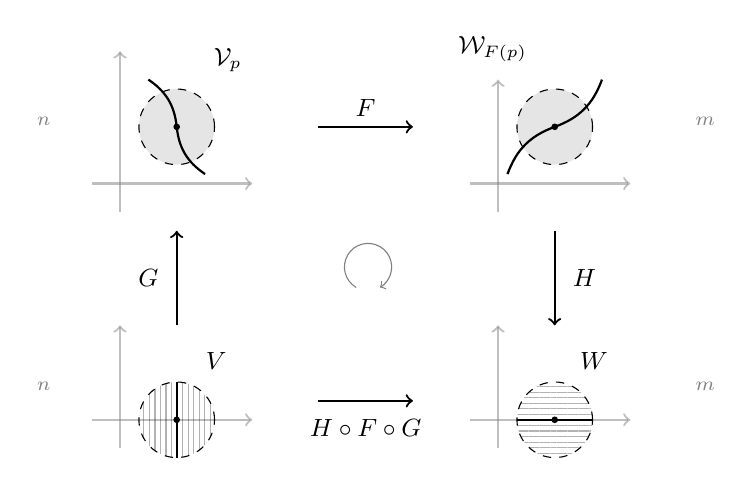
\begin{tikzpicture}[scale = 1.2, >=to]%, shift={(14.85cm,-0.9cm)}, baseline={(current bounding box.center)}, remember picture, overlay]
  % Puntos
  \coordinate (W) at (0,0); 
  % Espacio V
  \draw[thick]   (W) +(0.9,0.1) to[bend left= 25]  + (0.6,0.6);
  \draw[thick]   (W) + (0.6,0.6) to[bend left= -25]  + (0.3,1.1);
  \draw[->, thick, color = gray, opacity = 0.5]   (W)+(0,-0.3) --  + (0,1.4);
  \draw[->, thick, color = gray, opacity = 0.5]   (W) + (-0.3,0) --  +(1.4,0);
  \node[above, xshift = 0.65cm, yshift = -0.5cm] at ($(W) + (0.6, 1.5)$) {\small $\mathcal{V}_{p}$};
  \fill (W) + (0.6,0.6) circle (1pt);
  \draw[style=dashed, color = black]   (W) + (0.6,0.6) circle (0.4);
  \fill[color = black, opacity = 0.1]   (W) + (0.6,0.6) circle (0.4);
  \node[above, color = gray] at ($(W) + (-0.8,0.4)$) {$\R^n$};
  
  \coordinate (W) at (4,0); 
  % Espacio V
  \draw[thick]   (W) +(0.1,0.1) to[bend left= 25]  + (0.6,0.6);
  \draw[thick]   (W) + (0.6,0.6) to[bend left= -25]  + (1.1,1.1);
  \draw[->, thick, color = gray, opacity = 0.5]   (W)+(0,-0.3) --  + (0,1.1);
  \draw[->, thick, color = gray, opacity = 0.5]   (W) + (-0.3,0) --  +(1.4,0);
  \node[above, xshift = 0.65cm, yshift = -0.5cm] at ($(W) + (-0.6, 1.6)$) {\small $\mathcal{W}_{F(p)}$};
  \fill (W) + (0.6,0.6) circle (1pt);
  \draw[style=dashed, color = black]   (W) + (0.6,0.6) circle (0.4);
  \fill[color = black, opacity = 0.1]   (W) + (0.6,0.6) circle (0.4);
  \node[above, color = gray] at ($(W) + (2.2,0.4)$) {$\R^m$};

% BELOW
  \coordinate (W) at (0,-2.5); 
  % Espacio W
  \draw[->, thick, color = gray, opacity = 0.5]   (W)+(0,-0.3) --  + (0,1);
  \draw[->, thick, color = gray, opacity = 0.5]   (W) + (-0.3,0) --  +(1.4,0);
  \node[above, xshift = 0.5cm, yshift = -0.2cm] at ($(W) + (0.6, 0.6)$) {\small $V$};
  \fill (W) + (0.6,0) circle (1pt);
  \draw[thick] (W) + (0.6,-0.4) -- + (0.6, 0.4);
  \draw[style=dashed, color = black]   (W) + (0.6,0) circle (0.4);
  \fill[pattern={Lines[angle=90,distance=2pt,line width=0.4pt]},pattern color=black, opacity = 0.3]   (W) + (0.6,0) circle (0.4);
  \fill[];
  \node[above, color = gray] at ($(W) + (-0.8,0.1)$) {$\R^n$};

  \draw[->, thick] (W) + (0.6,1) -- +(0.6,2) node[midway, left, xshift = -0.1cm, yshift = 0cm] {\small $G$};
  \draw[->, thick] (W) + (4.6,2) -- +(4.6,1) node[midway, right, xshift = 0.1cm, yshift = 0cm] {\small $H$};

  \coordinate (W) at (4,-2.5); 
  % Espacio W
  \draw[->, thick, color = gray, opacity = 0.5]   (W)+(0,-0.3) --  + (0,1);
  \draw[->, thick, color = gray, opacity = 0.5]   (W) + (-0.3,0) --  +(1.4,0);
  \node[above, xshift = 0.5cm, yshift = -0.2cm] at ($(W) + (0.6, 0.6)$) {\small $W$};
  \fill (W) + (0.6,0) circle (1pt);
  \draw[thick] (W) + (0.2,0) -- + (1, 0);
  \draw[style=dashed, color = black]   (W) + (0.6,0) circle (0.4);
  \fill[pattern={Lines[angle=0,distance=2pt,line width=0.4pt]},pattern color=black, opacity = 0.3]   (W) + (0.6,0) circle (0.4);
  \fill[];
  \node[above, color = gray] at ($(W) + (2.2,0.1)$) {$\R^m$};
  % Flecha F
  \coordinate (W) at (2.9,-3.5); 
  \draw[->, thick] (2.1,0.6) -- (3.1,0.6) node[midway, above, xshift = -0cm, yshift = 0cm] {\small $F$};
  \draw[->, thick] (2.1,-2.3) -- (3.1,-2.3) node[midway, below, xshift = -0cm, yshift = -0.1cm] {\small $H\circ F\circ G$};
  \draw[->, color = gray, >=to] (2.5,-1.1) arc (240:-60:0.25);

\end{tikzpicture}
\caption{\(\blacksquare\) (Posto Constante)} 
\end{figure}

\begin{note}
    A função \(\operatorname{rank}: U \to \N\) é semi-continua inferiormente.
\end{note}

\begin{corollary}%[Colorarios]
  Os Teoremas de Função Inversa e Formas Locais (Imersões e Submersões) são diretos. Sejam \(F\in C^1(U;\R^m)\) e \(p\in U\). Então
  \begin{enumerate}[label = \roman*.]
    \item Se \(\operatorname{rank}(JF(p)) = r=\min \{n,m\}\) então \( \exists \mathcal{V}_p\) onde \(JF_r(\textbf{x}) \in GL_r(\R)\). 
    \item Se \(F\) é localmente injetiva então é imersão em \(V\ab\subset U\) denso em \(U\). \textcolor{gray}{\(\rightarrow \) Aplique \(\blacksquare\) (Posto Constante), a segunda afirmação segue da semi-continuidade inferior}
    \item Se \(F\) é aberta então é submersão em \(V\ab\subset U\) denso em \(U\). 
  \end{enumerate}
\end{corollary}

\alerta{
  \centering É preciso que o posto seja consta em TODA uma vizinhanza
  \tcblower
\begin{example}
  \(F: \R^2 \ni (t,s)\mapsto (t^2, t^3, s ) \in \R^3\) ¿Existem coordenadas como no Teorema em alguma vizinhanza de origem? \textcolor{gray}{\(\rightarrow \) Não} %\(\operatorname{rank}(JF(0,0))\)}
\end{example}
} 
\section{Variedades Differenciáveis}

\begin{definition}
    Sejam \(X\subseteq \R^n\) e \(Y\subseteq \R^m\), uma aplicação \(F\in C^k(X;Y)\) sse \(\forall p \in X\), \(\exists \widetilde{F} \in C^k(\U_p; \R^m)\) tal que \( \widetilde{F}|_{_{\U_p \cap X}} = F\).    
\end{definition}

%\begin{note}
%    Análogamente, se \(F \in C^\infty(X;Y)\), então dizemos que é \emph{suave}.
%\end{note}

\begin{definition}
    \(F: X \to Y\) é \emph{diffeomorfismo} de classe \(C^k\) se \(F\in C^k(X;Y)\) é homeomorfimso e \(F^{-1}\in C^k(Y;X)\). Denotamos \(^k F : X \simeq Y \). 
\end{definition}
\begin{example}
    Sejam \(X= \{(x,y) \in \mathbb{S}^1: y > 0 \}\) e \(Y = (-1,1)\). A aplicação \(\pi: X \ni (x,y) \mapsto x \in Y\) é \(^\infty F: X\simeq Y \). \textcolor{gray}{\(\rightarrow\) Verifique as condições}
\end{example}
\begin{definition}
    Um subconjunto \(^k_d M \subseteq \R^n\) é uma \emph{subvariedade} de classe \(C^k\) e dimensão \(d\), se  \(\forall p \in M \), \(\exists\ ^k \varphi: \U_p \cap M \simeq V\ab \subseteq \R^d\) \emph{carta local}, cujas componentes \(\varphi = (\x_1, \ldots, \x_d)\) são \emph{coordenadas locais} de \(M\) em \(p\). A inversa \(\varphi^{-1} = \psi : V \to \U_p \cap M \) é uma \emph{parametrização local} da variedade. 
\end{definition}

\begin{note}
    Por simplicidade na notação usaremos \(\U_p\) para indicar vizinhanza de \(p\) em \(M\) como subespaço de \(\R^n\). 
\end{note}

\begin{example}
    \(^{\infty}_{\hspace{0.15cm}n} U\ab\subseteq \R^n\). \textcolor{gray}{\(\rightarrow \) Tome \(\varphi = \id_n\)}
\end{example}
\begin{example}
    \(^{\hspace{0.3cm}\infty}_{n-1}\E^{n-1} \subseteq \R^n\). \textcolor{gray}{\(\rightarrow\) Construa a projeção estereográfica} 
\end{example}

\begin{lemma}
    Sejam \(^k_d M \subseteq \R^n \), \(V\ab\subseteq \R^d\) e \(\psi: V \to \R^n\) tal que \(\psi(V)\subseteq M \). Então, \(\psi\) é uma paremetrização local de \(M\) sse \(\psi \) é imersão e homeomorfismo (\(\tau_{_M}\)). 
\end{lemma}

\demo{(\(\Leftarrow\)) A bijeção é imediata de \(\psi(V)\ab \subseteq M\). Aplique \(\blacksquare\) (FLI) e faça a composição com a projeção. }

\alerta{\centering Imersão injetiva \textcolor{red}{\(\not\Rightarrow \)} homeomorfismo}

\begin{example}%[Coordenadas Esféricas]
    Parametrização local da esfera (coordenadas esféricas). Seja \(\psi: [0,\pi]^{n-2}\times [0, 2\pi) \to  \R^n\) tal que     
    \[(\theta_i) \mapsto \left(\cos\theta_1, \ldots, \prod^{j<i}\sin\theta_j \cdot \cos\theta_{i},\ldots, \prod\sin\theta_i\right). \] 
\end{example}
\begin{example}%[Gráficos]
    Se \(F\in C^k(U; \R^m)\) então \(\operatorname{graf}(F):= \{(\textbf{x},F(\textbf{x})) \in U\times\R^m\} = \ ^k_n M \subseteq \R^{n+m}\), com \(\psi: \textbf{x} \mapsto (\textbf{x}, F(\textbf{x}))\) e \(\varphi = \pi : (\textbf{x}, F(\textbf{x})) \mapsto \textbf{x}\).   
\end{example}
\begin{example}
    Seja \(^k H\subseteq \R^n\) hipersuperficie, então \(^{\hspace{0.5cm}k}_{n-1} H\subseteq \R^n\). \textcolor{gray}{\(\rightarrow\) \(H\) é localmente o gráfico de uma função} 
\end{example}

\begin{proposition}
    Seja \(G\in C^k(U;\R^m) \). Se \(\forall p \in U, \ G\) é submersão em \(p\), então \[\{p \in U : G(p)=0\} =:\ ^{\hspace{0.65cm}k}_{n-m}M \subseteq \R^n.\]     
\end{proposition}

%\begin{proposition}
%    \textcolor{rojoscuro}{\underline{\textbf{Exercise}}} \ Muestre que \(^k_d M\subseteq \R^n\) sii \(\forall p \in M, \ \exists \ ^kF: \U_p\simeq V\ab \) tal que \(F(\U_p\cap M ) = V \cap (\R^d \times \{0\}) = \{\textbf{y}\in V: \textbf{y} = (\textbf{y}^{(r)}, 0)\}\). 
%\end{proposition}

\begin{definition}
    Sejam \(^k_dM\subseteq \R^n\) e \(^k \psi_a: V\ab \simeq \U_p\) uma parametrização local tal que \(\psi_a(a)=p\). O \emph{espaço tangente} a \(p \in M \) é o dado por 
    \[T_pM := \operatorname{Im}(D\psi_a(a))= \bigoplus \R \frac{\partial \psi_a}{\partial x_i} (a)\leq \R^n. \]
\end{definition}

\begin{note}
    O espaço afim \(p + T_pM\) é o "intuitivamente" tangente a \(M\) en \(p\).
\end{note}

\begin{proposition}
    Sejam \(^k_d M \subseteq \R^n\) e \(c \in C^k(\V_\epsilon ; M)\) caminho em \(M\), então 
    \[T_pM = \{c'(0): c(0) =p \}. \] 
\end{proposition}

\begin{note}
    O espaço tangente não depende da parametrização.
\end{note}

\begin{example}
    Se \(U\ab\subseteq \R^n\) então \(T_pU= \R^n\). 
\end{example}
%\begin{example}
%    Se \(\psi(\alpha_1, \alpha_2)= p \in \E^2\) entonces  
%    \(T_p\E^2 = \R \frac{\partial \psi}{\partial \theta_1}(\alpha_1, \alpha_2)\oplus \R \frac{\partial \psi}{\partial \theta_2}(\alpha_1, \alpha_2)\). 
%\end{example}

%\begin{exercise}
%    Determine una parametrización del toro \(\mathbb{T}\subseteq\R^3\) y cálcule \(T_p\mathbb{T}\). 
%\end{exercise}

\begin{note}
    Em diante, para refererinos a \(^{\hspace{0.1cm}k}_{d_1}M\subseteq \R^n\) e \(^{\hspace{0.1cm}k}_{d_2}N\subseteq \R^m\) escrevemos simplesmente \(M\) e \(N\). %Dimensão, classe e espaço ambiente serão descritos apenas se fora necessario.
\end{note}

\begin{proposition}
    \(F\in C^k(M;N)\) sse \(\forall \psi: V\ab \to \U_p\) parametrização local de \(M\) em \(p\), tem-se que \(F \circ \psi \in C^k(V; N)\). \textcolor{gray}{\(\rightarrow\) Basta ver só um  atlas}  
\end{proposition}

\begin{definition}
    Seja \(F\in C^k(M;N)\). A derivada de \(F\) em \(p \in M\) é a aplicação linear \(DF(p): T_pM \to T_{F(p)}N \) tal que \( v\mapsto D\widetilde{F}(p) \cdot v\). 
\end{definition}

\begin{lemma}
    Se \(F\in C^k(M;N)\) então derivada \(DF(p)\) não depende da \(\widetilde{F}\).  
\end{lemma}

\demo{\parbox[a]{0.28\linewidth}{ }\parbox[b]{0.72\linewidth}{\vspace{0.3cm}Tome \(\psi_a\) e \(\psi_{b}{'}\) parametrizações locais de \(p\in M\) e \(F(p) \in N\). Faça \(\varphi{'} \circ F \circ \psi: V \to V{'}\), pelo \(\blacksquare\) (Regla da Cadeia) temos o diagrama a dereita. Note que \(D\widetilde{F}: \operatorname{Im}(D\psi_a(a))\mapsto \operatorname{Im}(D\psi_{a{'}}(a{'}))\). \vspace{0.3cm}}
}

\begin{tikzpicture}[scale = 1.2, >=to, shift={(11.95cm,1.5cm)}, baseline={(current bounding box.center)}, remember picture, overlay]
    
    \node (Up) at (0,0) { $\R^{d_1}$};
    \node (Rn) at (2.5,0) { $\R^{d_2}$};
    \node (Rn2) at (2.5,2) { $\R^n$};
    \node (U) at (0,2) { $\R^n$};
    
    %\node (c) at (3.6,0) {\footnotesize $L$};
    %\node (d) at (3.6,2) {\footnotesize$L^{-1}$};
    %\node (c1) at (3.6,1) {\rotatebox{90}{$\longmapsto$}};

    \draw[->] (Up) -- node[above, xshift = -0.45cm, yshift = -0.2cm] {\scriptsize \(\psi\)} (U);
    \draw[->] (Up) -- node[below] {\scriptsize \(D(\varphi{'}\circ F \circ \psi)\)} (Rn);
    \draw[->] (U) -- node[above] {\scriptsize \(DF\) } (Rn2);
    \draw[->] (Rn) -- node[right, xshift = 0.05cm, yshift = 0cm] {\scriptsize \(\psi{'}\)} (Rn2);
    \draw[->, color = gray, >=to] (1.15,0.85) arc (240:-60:0.25);

\end{tikzpicture}

\vspace{-1cm}

\begin{example}
    \(F: \E^1\to \E^1\) tal que \( (\cos\theta, \sin\theta) \equiv (x,y) \mapsto (x^2-y^2, 2xy) \equiv (\cos 2\theta, \sin 2\theta)\). \textcolor{gray}{\(\rightarrow \) Faça as contas }
\end{example}
%\begin{exercise}
%    Sea \(c \in C^k(\V_\epsilon; \R^m)\) tal que \(c(0)=p\). Muestre que si \(\vec{v} = c'(0)\in T_pM \) entonces \(DF(p)\cdot c{'}(0)= (F\circ c){'}(0)\). 
%\end{exercise}

\begin{note}
    Em geral, tudo o que foi visto para aplicações, vale em variedades: 
    \begin{description}
        \item[Regla da Cadeia] Se \(F\in C^k(M;N)\) e \(G \in C^k(N;P)\) então \(G \circ F \in C^k(M;P)\) e \(D(G\circ F)(p)  = DG(F(p))\cdot DF(p)\). 
        \item[Derivada da Identidade] \(D\id_{M} = \id_{T_pM}: T_pM \to T_pM\).  
        \item[Teorema da Função Inversa] Seja \(F\in C^k(M;N)\) tal que \(D\widetilde{F}(p)\) é isomorfismo, então \(\exists \ ^k F : \U_p\cap M \simeq \mathcal{V}_{F(p)} \cap N\).  
    \end{description}
\end{note}

\subsection{Valores Regulares}

\begin{definition}
    Seja \(F \in C^k(M;N)\). Um ponto \(p\in M\) é \emph{regular} se \(F\) é submersão em \(p\), se não fora regular então é \emph{ponto crítico} de \(F\).  
\end{definition}

\begin{note}
    Se \(\exists p\in M\) ponto regular de \(F\) então \(\dim M \geq \dim N\).
\end{note}

\ejemplo{ \centering \(\blacksquare\) (Multiplicadores de Lagrange)
\tcblower
\begin{example}
    Seja \(M= \ ^k H\subseteq \R^n\) hipersuperficie definida por \(g(\x)=0\) e \(f: \R^n \to \R\) função escalar, então 
    \[p \in M \text{ ponto crítico de } f(M) \textcolor{verdeoscuro}{\ \Leftrightarrow\  }df(p): T_pM \not \twoheadrightarrow \R.\]
\end{example}
}

%\{El multiplicador de Lagrange, de nuevo }

\begin{definition}
    Seja \(F\in C^k(M;N)\). Um valor \(q\in N\) é \emph{valor crítico} se \(\exists p\in M\) tal que \(p \) é ponto crítico de \(F\) e \(F(p)= q\), de outra forma é um \emph{valor regular} de \(F\).  
\end{definition}

\alerta{ \centering \(p\in M\) regular \textcolor{red}{\(\nRightarrow\)} \(q = F(p)\) regular}

\begin{note}
    Um conjunto da forma \(F^{-1}(q)\) é chamado \emph{fibra}.% ou "conjunto de nível". 
\end{note}

\begin{theorem}[\emph{Fibras Regulares}]
    Sean \(^{\hspace{0.1cm}k}_{d_1} M\subseteq \R^n\), \(^{\hspace{0.1cm}k}_{d_2}N\), \(F\in C^k(M;N)\). Si \(q \in N\) es un valor regular de \(F\), entonces \(P = F^{-1}(q)\) es \(^{\hspace{0.65cm}k} _{d_1 - d_2}P \subseteq M  \subseteq \R^n\).
\end{theorem}

\demo{Sejam \(p = F^{-1}(q)\) e \(d_1 - d_2 = c \). Note que \(\R^c \cong \ker DF(p) \leq \R^n\), defina \(L: \R^n \to \R^c\) tal que \(L\cdot \ker DF(p)\) é isomorfirsmo. Faça \(G:M \to N \times \R^c\) tal que \(\x\mapsto (F(\x), L(\x))\). Aplique \(\blacksquare\) (TFI) e conclua. }

\begin{example}
    \(1\) é valor regular de \(g: \R^n \ni \textbf{x}\mapsto  \sum x_i^2 \in \R\) e \(g^{-1}(1)= \E^{n-1}\). 
\end{example}

\ejemplo{ \centering Variedades de dimensão \(0\) 
\tcblower 
\begin{example}
    Sejam \(F\in C^k(M;N)\) com \(\dim M = \dim N \) e \(q \in N \) valor regular de \(F\). Então, \(P = F^{-1}(q)\) é um conjunto discreto. Ainda mais, se \(M\) fora compacto \(\Rightarrow |P| < \infty\). \textcolor{gray}{\(\rightarrow \ \R^0 = \{0\} \) }
\end{example}
}


%\begin{exercise}
%    Sea \(\mathcal{O}(n) := \{A \in GL_{n}(\R) : A A^T = \id_{n}\}\). Muestre que \(^{\hspace{0.8cm}k}_{n(n-1)} \mathcal{O}(n) \subseteq \R^{n^2}\). Cálcule \(T_{\id_{n}}(\mathcal{O}(n))\) y verifique sin es un conjunto conexo. 
%\end{exercise}

%\begin{exercise}[Fibras de Rango Constante]
%    Sea \(F\in C^k(M;N)\) e \(F^{-1}(q) \subseteq \ ^{\hspace{0cm}k}_{d}M\subseteq \R^n\) tal que \(\exists \ \U_{F^{-1}(q)}\) donde \(\operatorname{ran}(DF(\textbf{x})) = r\), entonces \(^{\hspace{0.35cm}k}_{d - r}F^{-1}(q)\subseteq M \subseteq \R^n\). 
%\end{exercise}
%\begin{note}
%    ¿Que se puede decir de los valores regulares?
%\end{note}

\begin{theorem}[\emph{Brown-Sard}]
    Seja \(F\in C^k(M;N)\). Se \(k \gg 0\) então o subconjunto de valores regulares de \(F\) é denso em \(N\).% \footnote{Se exige \(k\geq \dim M - \dim N + 1\) pero así se ve mas bonito }
\end{theorem}

\begin{note}
    A medida de \(B= (a_i,b_i)^n\subseteq \R^n\) bloque aberto é \(\mu(B):= \prod (b_i-a_i)\).
\end{note}

\begin{definition}
    Um subconjunto \(S\subseteq \R^n\) tém \emph{medida nula} se \(\forall \epsilon >0\),  \(\exists B_i\) bloques abertos tais que  \(S\subseteq \bigcup B_i\) e \(\sum \mu(B_i)< \epsilon\). .  
\end{definition}

\begin{example}
    Se \(n<m\) então \(\R^n\times \{0\}\subseteq \R^m\) tém medida nula.   
\end{example}
\begin{example}
    \(S\subseteq \R^n\) enumerável tém medida nula.  \textcolor{gray}{\(\rightarrow\) Pontos isolados} 
\end{example}
\begin{theorem}[\emph{Sard}]
    Sejam \(U\ab\subseteq \R^n\) e \(F\in C^k(U; \R^m)\) tal que \(k\geq \{n-m+1, 1\}\). Então, o conjuntos de valores críticos de \(F\) tém medida nula em \(\R^n\). 
\end{theorem}

\begin{example}
    Pelo \(\blacksquare\) (Sard) \  \(^k_d M\subseteq \R^n\) com \(d<n\) tém medida nula. \textcolor{gray}{\(\rightarrow\) Todos os valores da inclusão \(\iota : M \hookrightarrow \R^n\) são críticos}
\end{example}

\begin{exercise}
    Se \(S\subseteq \R^n \) tém medida nula então \(\R^n\setminus S \) é denso. 
\end{exercise}


\section{Formas Differenciais}

\ejemplo{
    Nosso objetivo é uma noção geral de integral em variedades que não dependa da escolha da parametrização local.
    \tcblower
\begin{example} \- \vspace{-0.5cm}
    \[\int_a^b \overbrace{f(t) \ dt}^{\overset{\text{Forma Diff}}{\uparrow}}  \ \ \ \overset{^{t\to 2u}}{=}\ \ \  \int_{\frac{a}{2}}^{\frac{b}{2}} f(2u)  \ 2du. \]
\end{example}
}

\subsection{Formas Alternadas}

\begin{definition}
    Seja \(V\) espaço vectorial. Uma $k$-\emph{forma} alternada é uma função \(k\)-linear, \(\alpha: V^k \to \R\) tal que, se \(v_i = v_j\) para algum \(i\neq j\) então \(\alpha(v_1, \ldots, v_k) = 0\). 
\end{definition}

\begin{example}
    \(\alpha: V \to \R\) linear é \(1\)-forma alternada. \textcolor{gray}{\(\rightarrow\) A antissimetria é trivial}
\end{example}

\begin{note}
    \(V^0 = \{\emptyset\}\), logo, uma $0$-forma é simplesmente um \(\alpha(o) \in \R\). 
\end{note}

\parbox[l]{0.7\linewidth}{

\begin{example}
    A função \(\det : (\R^2)^2 \to \R\) é \(2\)-forma alternada em \(V= \R^2\), onde 
    \[\begin{pmatrix}
        a \\ b
    \end{pmatrix}\times \begin{pmatrix}
        c \\ d
    \end{pmatrix} \mapsto \det\begin{pmatrix}
        a & c \\ 
        b & d
    \end{pmatrix}.\]  
\end{example}
}

\begin{tikzpicture}[>=to, shift={(14.4cm,2.7cm)}, baseline={(current bounding box.center)}, remember picture, overlay, scale = 0.75]
    % Definimos los vectores v1 y v2
    \coordinate (O) at (0,0);
    \coordinate (v1) at (3.5,0);
    \coordinate (v2) at (1,2);
    
    % Calculamos los otros vértices del paralelogramo
    \coordinate (v1v2) at ($(v1) + (v2)$);
    
    % Sombra del área
    \fill[gray!10] (O) -- (v1) -- (v1v2) -- (v2) -- cycle;
    %\fill[pattern={Lines[angle=0,distance=4pt,line width=0.4pt]},pattern color=gray] (O) -- (v1) -- (v1v2) -- (v2) -- cycle;
    \node[thick] at (2,1.02) {\textbf{$P$}};
    \draw[->, thick] (2.1,0.65) arc (-90:55:0.4);
    % Dibujo de los lados
    \draw[thick, gray!23] (O) -- (v1) -- (v1v2) -- (v2) -- cycle;

    % Dibujo de los vectores
    \draw[->, black, thick] (O) -- (v1) node[midway, below, yshift = -0.05cm] {$v_1$};
    \draw[->, black, thick] (O) -- (v2) node[midway, above left ] {$v_2$};

    % Ejes
    \node at (1.7,-1.6) { \rotatebox{-90}{\large$\rightsquigarrow$}};
    \node at (2.3,-1.6) { $\alpha$};
%    \node at (2.1,-1.6) {\LARGE \rotatebox{-90}{$\rightsquigarrow$}};
    \draw[<->, gray] (-0,-2.4) -- (3.5,-2.4) node[above right] {\textcolor{black}{$\R$}};
    \fill[thick] (1.76,-2.4) circle (2pt);
    %\draw[->, gray] (0,-0.5) -- (0,3) node[above] {$y$};
\end{tikzpicture}

\- \vspace{-2cm} 
\begin{note}
    A função \(\alpha\) é tipo um "volume" \(k\)-dimensional com sinal, dada pela "orientação" ou ordem de os \(v_i\). 
\end{note}

\begin{definition}
    \centering \(A^k(V):=\{\alpha \ | \ \alpha \text{ é } k\text{-forma alternada}\}\)
\end{definition} 
%\begin{note}
%    \(A^k(V)\) es espacio vectorial.
%\end{note}% al espacio vectorial de todas las $k$-formas definidas en \(V\).  

\begin{lemma}
    Seja \(\alpha \in A^k(V)\) e \(i<j\). Então,  
    \begin{enumerate}[label = \roman*.]
        \item \(\alpha (v_1, \ldots, v_i, \ldots, v_j, \ldots, v_k) = -\alpha (v_1, \ldots, v_j, \ldots, v_i, \ldots, v_k)\).
        \textcolor{gray}{\(\rightarrow \) Denote \(\alpha(v_i,v_j)\) e faça a conta \(0=\alpha(v_i+v_j, v_i+v_j)\)}
        \item Se \(v_1, \ldots, v_k\) são l.d. então \(\alpha (v_1, \ldots, v_k) = 0\). \textcolor{gray}{\(\rightarrow\) Expresse \(v_1 = \sum \lambda_jv_j\) e faça a conta}
    \end{enumerate}
\end{lemma}

\begin{corollary}
    As formas alternadas são antisimetricas. Se \(S_k\) é o grupo de permutações de ordem \(k\) e \(\operatorname{sgn} : S_k \ni \sigma \mapsto \operatorname{sgn}(\sigma) \in \{-1, 1\}\) então,
    \[\alpha(v_{\sigma(1)}, \ldots, v_{\sigma(k)}) = \operatorname{sgn}(\sigma) \cdot \alpha(v_1, \ldots, v_{k}) .\] 
\end{corollary}

\begin{note} 
    \(S_k \ni \sigma = \prod \tau_j : \tau_j\) é transposição, assim, \(\operatorname{sgn}(\sigma) = (-1)^{|J|}\).
\end{note}

\ejemplo{\centering Espaços não triviais \( \sim \ \dim V = n\)
\tcblower 
\begin{example}
    \(A^0(V) = \R \), \(A^1(V) = V^*\) e \(A^k(V) = \{0\}\) se \(k > n\). \textcolor{gray}{\(\rightarrow \) Segue de o lemma sobre dependencia linear}
\end{example}
}

\begin{exercise}[Projetor Alternado]
    Seja \(f: V^k \to \R\) função $k$-linear, então 
    \[Af :  (v_1, \ldots, v_k) \mapsto \frac{1}{k!} \sum_{\sigma} \operatorname{sgn}(\sigma) f(v_{\sigma(1)}, \ldots, v_{\sigma(k)}),\] 
    é uma $k$-forma alternada. Em particular, se \(f\) é alternada, então \(Af = f \). 
\end{exercise}

\begin{definition}
    Sejam \(T \in \mathcal{L}(V;W)\) e \(\alpha \in A^k(W)\). O \emph{pullback} de \(\alpha \) por \(T\) é a função \(T^*\alpha: V^k \to \R\) tal que \((v_1, \ldots, v_k) \mapsto \alpha (Tv_1, \ldots, Tv_k)\). 
\end{definition}

\ejemplo{
 \centering   \(T^* : A^k(W)\to A^k(V)\)
    \tcblower
\begin{example}
    \(\pi: \R^3 \ni (x,y,z) \mapsto (x,y) \in \R^2\) e \(\det \in A^2(\R^2)\) então, 
\vspace{-0.3cm}
    \[\pi^*\alpha ((x,y,z), (x{'}, y{'}, z{'})) = \alpha( (x,y), (x{'}, y{'})) = \det \begin{pmatrix}
        x & x{'}\\ 
        y & y{'}
    \end{pmatrix}. \] 
\end{example}
}

\let\originalwedge\wedge 
\renewcommand{\wedge}{\mathbin{\scriptstyle\originalwedge}}

\begin{definition}
    Sejam \(\alpha \in A^p(V)\) e \(\beta \in A^q(V)\). O \emph{produto exterior} de \(\alpha\) e \(\beta\) é a função \(\alpha \wedge \beta : V^{p+q} \to \R\) dada por,  
    {\[(v_1, \ldots, v_{p+q}) \mapsto \frac{1}{p!q!} \sum_\sigma \operatorname{sgn}(\sigma) \alpha(v_{\sigma(1)}, \ldots, v_{\sigma(p)}) \beta(v_{\sigma(p+1)},\ldots, v_{\sigma(p+q)}).\]}
\end{definition}

\begin{example}
    Sejam \(\alpha, \beta \in A^1(V)\). Então,  \(\alpha \wedge \beta \in A^2(V)\) é a dada por
    \vspace{-0.2cm}
    \[(v_1, v_2) \mapsto \alpha(v_1)\beta(v_2) - \alpha(v_2)\beta(v_1) =\det  \begin{pmatrix}
        \alpha(v_1) & \beta(v_1) \\ 
        \alpha(v_2) & \beta(v_2) 
    \end{pmatrix}.\] 
\end{example}

%\begin{example}
%    \(\Lambda^0(\R^2) = \R\), \(\Lambda^1(\R^2) = \R e_1^* \oplus \R e_2^*\) e \(\Lambda^2(\R^2) = \R (e_1^* \wedge e_2^*)\).   
%\end{example}

\begin{proposition}
    Sejam \(\alpha \in A^p(V),\ \beta \in A^q(V)\) e \(\gamma \in A^r(V)\). Então, o produto \(\wedge\) é:   
    \begin{enumerate}[label = \roman*.]
        \item \(A^p(V) \times A^q(V) \ni (\alpha, \beta )\to \alpha \wedge \beta \in A^{p+q}(V)\), bém definido.   
        \item Bilinear, se \(p = r \Rightarrow (\alpha + \lambda \gamma) \wedge \beta =  \alpha \wedge \beta + \lambda (\gamma \wedge \beta)\), na outra coordenada, se \(q = r \Rightarrow \alpha  \wedge (\beta+ \lambda \gamma) =  \alpha \wedge \beta + \lambda (\alpha \wedge \gamma) \). %\textcolor{gray}{\(\rightarrow \) ii. e v. Directos de la definición} 
        \item Anticonmutativo, \(\alpha \wedge \beta =  (-1)^{pq} \beta \wedge \alpha\). \textcolor{gray}{\(\rightarrow \) Tome a permutação \[\begin{pmatrix}
    1\ \ \ \cdots \ \ \  p & p+1  \cdots  p+q\\ 
    q+ 1 \cdots  q+p & 1 \ \ \  \cdots \ \ \  q
\end{pmatrix}\] }
        \item Associativo, \((\alpha \wedge \beta) \wedge \gamma = \alpha \wedge (\beta \wedge \gamma)\). \textcolor{gray}{\(\rightarrow \) Use o projetor alternado em \(f(v_i), \ i \in \{n\in \N : n\leq p+q+r\}\) e faça as contas chatas}
        \item Compativél com pullback, \(T^*(\alpha \wedge \beta) = T^*\alpha \wedge T^*\beta\).   
    \end{enumerate} 
\end{proposition}

\begin{theorem}
    Sejam \(V\) espaço vectorial e \([l_1, \ldots, l_n]\) uma base l.i. Então, \(\forall k\leq n \), temos que \(A^k(V) = [l_{i_1}\wedge \cdots \wedge l_{i_k}]\). Em particular, \(\dim A^k(V) = \binom{n}{k}\).   
\end{theorem}

%\ejemplo{\centering Pullback de cambio de base%
%\tcblower
\begin{example}
    Se \(V = [\omega_1, \ldots, \omega_n]\) (l.i.) e \(\alpha \in A^n(V)\) então, \(\alpha(v_1, \ldots, v_n) = \det(a_{ij}) \alpha(\omega_1, \ldots, \omega_n)\), onde \(v_j = \sum a_{ij}\omega_i\). \textcolor{gray}{ \(\rightarrow \ T^*\alpha = \det(T)\alpha\)}  
\end{example}
%}

\begin{example}
    \- \vspace{-1cm}
    \[(\R^3)^{*} = [e_1^*, e_2^*, e_3^*] \leadsto  \begin{cases}
        A^0(\R^3) = \R\\ 
        A^1(\R^3) = \R e_1^* \oplus \R e_2^*\oplus\R e_3^*\\ 
        A^2(\R^3) = \R (e_1^* \wedge e_2^*)\oplus \R (e_1^* \wedge e_3^*)\oplus \R (e_2^* \wedge e_3^*)\\ 
        A^3(\R^3) = \R ( e_1^* \wedge e_2^*\wedge e_3^*) \sim \det(\R^3) \\ 
    \end{cases}\]   
\end{example}

\subsection{Formas Differenciais}



\begin{note}
    Se \( \varphi = (\x_1, \ldots, \x_d): \U_p \to \R^d\) é uma carta local de \(^r_dM \subseteq \R^n\), lembre-se que \([d\x_1, \ldots, d\x_d]  = (T_pM)^* = A^1(T_pM)\). %Também, \(A^k(T_pM) = [d\x_{i_1}\wedge \cdots \wedge d\x_{i_k}]\). 
\end{note}
\- \vspace{-0.8cm}
\begin{definition}
    Uma \emph{$k$-forma diff} de classe \(C^r\) em \(^r_dM\subseteq \R^n\), é uma associação 
    \[^r_k\omega : M \ni p \mapsto \omega(p) = \sum f_{i_1, \ldots, i_k} \ d\x_{i_1}\wedge \cdots \wedge d\x_{i_k} \in A^k(T_pM), \] 
    tal que, \(\forall \varphi = (\x_1, \ldots, \x_d)\), as funções \(f_{i_1, \ldots, i_k}\in C^r ( \U_p;\R)\).
\end{definition}

%\ejemplo{Basta probar para un único atlas }

\begin{note}
    Em deante tudo será \(C^\infty\), variedades, aplicações, formas, etc. 
\end{note}

\begin{definition}
    \centering \(\Omega^k(M):= \{ \omega \ | \ \omega \text{ é } k\text{-forma diff}\}\)  
\end{definition}

\ejemplo{ %\centering \(_nM = U\ab\subseteq \R^n\) e \(dx_i = e_i^*\)
%\tcblower
\- \vspace{-0.6cm}
    \[\sum f_{i_1, \ldots, i_k} \ dx_{i_1}\wedge \cdots \wedge dx_{i_k} = \omega  \in \Omega^k(U\ab) \ \textcolor{verdeoscuro}{\Leftrightarrow} \ f_{i_1, \ldots, i_k} \in C^\infty(U)\]
    \tcblower
        {\footnotesize \(\bullet\)} Se \(U = I\subset \R \), então \(\omega = f(t)  dt \in \Omega^1(I)\) sse \(f \in C^\infty(I)\).    \\ 
        %\item Si \(M = U\ab \subseteq \R^2\) de coordenadas \((x,y)\) entonces,  
        {\footnotesize \(\bullet\)} Se \( U\subseteq \R^2 \) e \(f,g \in C^\infty( U)\) então 
        \(f \in \Omega^0(U),  \  f dx + g dy \in \Omega^1(U) \text{\  e}  \ f (dx \wedge dy) \in \Omega^2(U)\). 
}

\begin{note}
    Em geral, \(\Omega^0(M)=C^\infty(M;\R)\) e se \(f \in C^\infty(M; \R)\) então \(df \in \Omega^1(M)\), pois, \(df(p)\in (T_pM)^* = A^1(T_pM)\).    
\end{note}

\begin{exercise}
    Seja \(\varphi = (\x_1, \ldots, \x_d) : \U_p \to \R^d\) carta local de \(_dM\), então 
    \[df\Big|_{\U_p} = \sum \frac{\partial f }{\partial \x_i} \ d\x_i, \ \text{sendo }  \frac{\partial f }{\partial \x_i}(p) := \frac{\partial }{\partial t_i} (f\circ \varphi^{-1})(\varphi(p)).\]
    Onde, \((t_1, \ldots, t_d)\) são as coordenadas canônicas de \(\R^d\).  
\end{exercise}

\ejemplo{
\centering \((\omega \wedge \eta)(p) = \omega (p) \wedge \eta (p)\) 
\tcblower
\begin{example}
    Em \(M= \R^2\), tém-se \((e^{x+y}dx + x dy) \wedge (y dx) = -xy \ (dx \wedge dy)\). 
\end{example}
}

\begin{proposition}
    Uma aplicação \(F\in C^\infty(M;N)\) induce, \(\forall p \in M\), uma outra aplicação via pullback \(F^*: \Omega^k(N) \to \Omega^k(M)\)  tal que, 
    \[  \omega\textcolor{gray}{(p)} \mapsto F^*\omega \textcolor{gray}{(p)} = DF\textcolor{gray}{(p)}^*\omega(F\textcolor{gray}{(p)}).\] 
\end{proposition}
\vspace{-0.4cm}

\begin{example}
    Se \(g \in \Omega^0(N)\) então \(F^*g = g \circ F\) e \(F^*(dg) = d(F^*g) = d (g\circ F)\).   
\end{example}

\begin{tikzpicture}[>=to, shift={(7.3cm,-3.5cm)}, baseline={(current bounding box.center)}, remember picture, overlay]
    \draw[thick, red] (1.3,-0.3) -- (1.3,0.3) -- (5.3,0.3); 
    \node[red] at (8.5,0.3) {$F^*\y_{i_1} = \sum \frac{\partial F^*\y_{i_1}}{\partial \x_j}d\x_j $};
\end{tikzpicture}

\vspace{-1cm}

\begin{note}
    Na hora das contas, se \(\varphi = (\x_1, \ldots, \x_{d_1})\) e \(\varphi{'}(\y_1, \ldots, \y_{d_2})\) são cartas locais de \(p\) e \(F(p)\) respetivamente, tais que \(F(\U_p)\subseteq \mathcal{V}_{F(p)}\), então 
    \begin{align*}
        \omega\Big|_{\mathcal{V}_{F(p)}} &=  \underset{\rotatebox{-90}{$\Rightarrow$}}{\sum} g_{i_1, \ldots, i_k} d\y_{i_1} \wedge \cdots \wedge d\y_{i_k} \\  
        (F^*\omega )\Big|_{\U_p} = \sum &F^*g_{i_1, \ldots, i_k} d(\textcolor{red}{F^*\y_{i_1}} ) \wedge \cdots \wedge d(F^*\y_{i_k})  \hspace{4cm}
    \end{align*}
\end{note}
 
Em particular, se \(F = \iota: M \to N\) então \(\iota^*\omega = \omega|_{_M}\).

\begin{example}
    Sejam \( \omega = fdx + g dy \in \Omega^1(\R^2)\) e \(c: I\subset \R \to \R^2\) uma curva suave, então \(c^*\omega = (f(c(t))c_1{'}(t) + g(c(t))c_2{'}(t)) dt\).  
\end{example}

\begin{example}[Forma de angulo]
    \(\displaystyle d\theta = \frac{y dx - xdy }{x^2+ y^2} \in \Omega^1(\R^2\setminus\{0\})\). 
\end{example}

%\ejemplo{\ \(\iota: \E^1 \to \R^2 \setminus \{0\} \Rightarrow d\theta|_{_{\E^1}} \in \Omega^1(\E^1)\)}

\begin{definition}
    Uma variedade \(_dM\) é \emph{orientavél} se \(\exists \omega \in \Omega^d(M)\), chamada \emph{forma de orientação}, tal que \(\forall p \in M, \ \omega(p)\neq 0 \). 
\end{definition}

\begin{example}
    \(\R^n\) é orientavél com \(\omega = dx_1 \wedge \cdots \wedge dx_n\) e \(\E^1\) com \(\omega = d\theta\Big|_{_{\E^1}}\).
\end{example}
\begin{example}
    A faixa de Möbius não é orientavél. 
\end{example}

\begin{definition}
    Sejam \(M\) orientavél e \(\omega, \omega{'} \in \Omega^d(M)\) formas de orientação.  Então, \(\omega \sim \omega{'}\) se \(\exists f>0\) tal que \(\omega = f \omega{'}\). Uma \emph{orientação} de \(M\) é \([\omega]/\hspace{-0.1cm}\sim\). 
\end{definition}

\begin{exercise}
    Se \(M\) é conexa e orientavél então tém só dois orientações. %\(\operatorname{card}(\Omega^d(M) /\hspace{-0.1cm} \sim) = 2 \).
\end{exercise}

\begin{definition}
    Seja \(M\) orientavél. A \emph{forma de volume} de \(M\) é a única representante \(\omega_\text{vol}\) de \([\omega]\in \Omega^d(M)/\hspace{-0.1cm}\sim\), tal que, \(\forall [w_1, \ldots, w_d]\) base ortonormal de \(T_pM\), 
    \[\omega_\text{vol}(w_1, \ldots, w_d) = 1 \ \ \text{e} \ \ \omega(w_1,\ldots, w_d) > 0.\] 
\end{definition}

\begin{example}
    \(\omega_\text{vol} = dx_1 \wedge \cdots \wedge dx_n\) é a forma de volume de \(\R^n\). 
\end{example}

\ejemplo{\centering  \(\omega_\text{vol}\) em \(_{n-1}H\subseteq \R^n\) hipersuperficie
\tcblower
\parbox[a]{0\linewidth}{ \ } 
\parbox[b]{1\linewidth}{
\begin{example}
    \(H := \{\x \in \R^n: g(\x)=0\}\) é orientavél. Sendo \(\vec{n}(p) = \frac{\nabla g(p) }{\|\nabla g(p)\|} \perp  T_pH\), sua forma de volume é
    \[\omega_\text{vol} = \sum (-1^{i+1}) \vec{n_i} \  d\x_1\wedge \cdots \wedge \textcolor{gray}{\widehat{d\x_i}} \wedge \cdots \wedge d\x_n \Big|_{H}.\hspace{4.5cm}\]     
\end{example}
} 
}

\begin{tikzpicture}[>=to, shift={(15.8cm,2.8cm)}, baseline={(current bounding box.center)}, remember picture, overlay]
    \node[gray] at (0,0) {\footnotesize$\det \begin{pmatrix}
        \textcolor{red}{\Big|} &\Big| &  &\Big| \\ 
        \textcolor{red}{\vec{n}}& v_2 & \cdots &v_n \\ 
        \textcolor{red}{\Big|} &\Big| &  &\Big|
    \end{pmatrix}$};  
\end{tikzpicture}

%\begin{tikzpicture}[>=to, shift={(2.9cm,1.5cm)}, baseline={(current bounding box.center)}, remember picture, overlay]
%    \draw[thick] (0,0) -- (0,0.25) -- (10.8,0.25); 
%\end{tikzpicture}

\vspace{-1cm}

\begin{example}
    Em \(H = \E^{n-1}\subseteq \R^n\) temos \(\vec{n}(x) = \frac{\x}{\|\x\|}\), logo, 
    \[\omega_\text{vol} = \sum (-1)^{i+1} x_i \ d\x_1 \wedge \cdots \wedge \textcolor{gray}{\widehat{d\x_i}} \wedge \cdots \wedge d\x_n\Big|_{\E^{n-1}}.\]
\end{example}

%\begin{exercise}
%    Faça \(\psi^*\omega_\text{vol}\) de \(\E^{n-1}\), com \(\psi\) sendo as coordenadas esféricas.  
%\end{exercise}

\subsection{Derivada Exterior}

\begin{note}
    A idea agora é entender como se derivam as formas diferenciais. 
\end{note}

\begin{theorem}
    \(\forall M, \ \forall k \in \N\), \(\exists !d_i \in \mathcal{L}(\Omega^k(M) ; \Omega^{k+1}(M))\), onde \(d_i: \omega \mapsto d\omega\) verifica,  
    \begin{enumerate}[label= \roman*.]
        \item Derivada de uma função, \(\Omega^0(M) = C^\infty(M) \ni f \mapsto df \in \Omega^1(M)\). 
        \item Regla de Leibniz com sinal, se \(\omega \in \Omega^p(M)\) e \(\eta\in \Omega^q(M)\) então, 
        \[ d(\omega \wedge \eta ) = d\omega \wedge \eta + (-1)^p \omega \wedge d \eta. \]
        \item \(d^2 =0\), se \(\omega \in \Omega^k(M)\) então \(d (d\omega) = 0\). \textcolor{gray}{\(\rightarrow \) Motivada pelo \(\blacksquare\) (\emph{Schwarz})}
        \item Compativél com pullback, se \(F \in C^\infty (M;N)\) e \(\omega \in \Omega^k(N)\) então, 
        \[d(F^*\omega) = F^*(d\omega).\] 
    \end{enumerate}
\end{theorem}



\begin{example}
    Sendo \(I = (i_1, \ldots, i_k)\) e \(\sum f_{I} \  d\x_{I} = \omega \in \Omega^k(M)\), temos,     
    \begin{equation*}
        d\omega = \sum   df_I \ d\x_I. 
    \end{equation*} 
\end{example}
%\ejemplo{\(\rightarrow\) Desarme usando las propiedades del Teorema previo. Siendo  tenemos,\[d\left(\sum f_I d\x_I\right) = \sum df_I d\x_I\]. En este caso, la condición \(d^2= 0 \) se traduce en \(\operatorname{rot}\circ \nabla = 0 = \operatorname{div}\circ \operatorname{rot}\)}
%\begin{figure}[!h]
%    \centering     
%\begin{tikzpicture}[>=stealth]
%
% Nodos fila superior
%\node (A1) at (0,1.5) {$\Omega^0(U)$};
%\node (A2) at (2.5,1.5) {$\Omega^1(U)$};
%\node (A3) at (5.5,1.5) {$\Omega^2(U)$};
%\node (A4) at (8,1.5) {$\Omega^3(U)$};

% Nodos fila inferior
%\node (B1) at (0,0) {$C^\infty(U)$};
%\node (B2) at (2.5,0) {$C^\infty(U;\R^3)$};
%\node (B3) at (5.5,0) {$C^\infty(U;\R^3)$};
%\node (B4) at (8,0) {$C^\infty(U)$};

% Flechas horizontales fila superior (e)
%\draw[->] (A1) -- (A2) node[midway, above] {$d$};
%\draw[->] (A2) -- (A3) node[midway, above] {$d$};
%\draw[->] (A3) -- (A4) node[midway, above] {$d$};
%
% Flechas horizontales fila inferior (e)
%\draw[->] (B1) -- (B2) node[midway, below] {\footnotesize$\nabla$};
%\draw[->] (B2) -- (B3) node[midway, below] {\footnotesize$\operatorname{rot}$};
%\draw[->] (B3) -- (B4) node[midway, below] {\footnotesize$\operatorname{div} $};

% Flechas verticales (w)
%\draw[->,white] (A1) -- (B1) node[midway, left, xshift = 0.2cm] {\textcolor{black}{\rotatebox{-90}{$\cong$}}};
%\draw[->,white] (A2) -- (B2) node[midway, left, xshift = 0.2cm] {\textcolor{black}{\rotatebox{-90}{$\cong$}}};
%\draw[->,white] (A3) -- (B3) node[midway, left, xshift = 0.2cm] {\textcolor{black}{\rotatebox{-90}{$\cong$}}};
%\draw[->,white] (A4) -- (B4) node[midway, left, xshift = 0.2cm] {\textcolor{black}{\rotatebox{-90}{$\cong$}}};

%\end{tikzpicture}
%\caption{\(_3M= U\ab\subseteq \R^3\)}
%    \end{figure}

\vspace{-0.5cm}
\begin{definition}
    \(\omega \in \Omega^k(M)\) é \emph{exata} se \(\exists \eta \in \Omega^{k-1}(M)\) tal que \(\omega = d\eta\). Por outro lado, se \(d\omega = 0 \) dezimos então que é \emph{fechada}. 
\end{definition}
\begin{note}
    Ver que \(\omega \) é exata é "resolver" EDPs, ou seja integrar.
\end{note}
%\begin{exercise}
%    Muestre que \(d\theta \in \Omega^1(\R^2\setminus \{0\})\), es cerrada, pero no exacta. \textcolor{gray}{\(\rightarrow\) Es exacta solo en abiertos de la forma \(\R^2\setminus  (-\infty, 0]\)} 
%\end{exercise}
\section{Integração em Variedades}

\begin{note}
    Nesta seção \(I = [0,1]\subset \R\). 
\end{note}

\subsection{Integração em Cadeias}

\begin{definition}
    Um \(k\)\emph{-bloco singular} em \(M\) é uma aplicação \(\sigma \in C^\infty(I^k; M)\).
\end{definition}

%\ejemplo{ \centering  
%    \tcblower
\begin{example}[$n$-bloco padrão em \(\R^n\)]
    \(\id_{I^n} : I^n \to I^n \subset \R^n \). 
\end{example}
%}
\begin{example}%[$n$-bloco padrão em \(\R^n\)]
    Uma curva suave \(c : I \to M \) é um \(1\)-bloco singular. 
\end{example}

\alerta{
\centering \(\sigma \  \ k\)-bloco singular \(\textcolor{red}{\neq}  \ \ \operatorname{Im}(\sigma)\subseteq M\) 
\tcblower
\begin{example}
    \(\sigma: I^n \ni \x \mapsto p \in M \) é um $n$-bloco singular.%, chamamos ele em particular de $n$\emph{-cubo singular}. 
\end{example}
}

\begin{definition}
    Sejam \(\omega \in \Omega^k(M)\) e \(\sigma \) um $k$-bloco singular. Então,  
    \[\int_\sigma \omega = \int_{I^k} \sigma^*\omega = \int_{I^k}f(\x) \ dx_1\wedge \cdots \wedge dx_k =\int_{I^k} f(\x) \ d\x. \]  
\end{definition}

\ejemplo{
\centering Integral de linha
\tcblower
\begin{example}
    Sejam \(c(t) : [a,b] \to U\ab\subseteq \R^n\) curva suave e \(\overset{n}{\sum} f_i \ dx_i = \omega \in \Omega^k(U) \), então temos
    \[\oint_c \omega = \int_a^b c^*\omega \ dt = \int_a^b \sum^n (f_i \circ c)(t) c_i{'}(t) \ dt\]
\end{example}
}

%\parbox[l]{0.6\linewidth}{
\begin{definition}
    Uma $k$\emph{-cadeia} de blocos singulares em \(M\) é uma expresão da forma 
    \[ c = \overset{k}{\sum} n_i \sigma_i, \ n_i \in \mathbb{Z} \ \text{e } \sigma_i:I^k\to  M.\] 
    %onde \(n_j \in \mathbb{Z} \) e \(\sigma_j: I^k \to M \) é um $k$-cubo singular.
\end{definition}
%}
\vspace{0.3cm}
\begin{example}
 \(c = 2c_1 + c_2 \textcolor{red}{-} c_3\).    
\end{example}

\- \vspace{-1cm}
\begin{tikzpicture}[>=to, shift={(8.25cm,-1.1cm)}, baseline={(current bounding box.center)}, remember picture, overlay]
  % Dibuja la cuadrícula de puntos

  % C1
  \draw[thick] (0.5,2.5) to[out=-20, in=180] (2.5,3) node[yshift = 3cm, xshift=1cm, midway, above] {$c_1$};
    \fill (0.5,2.5) circle (2pt);
  % C2
  \draw[thick] (2.5,3) to[out=-45, in=170] (4,2) node[yshift = 2.5cm, xshift=3.7cm, midway, above] {$c_2$};
    \fill (2.5,3) circle (2pt);
    \fill (4,2) circle (2pt);

  % C3
  \draw[red] (5,2.5) to[out=60, in=225] (5.7,3.5) node[yshift = 2.3cm, xshift=6cm, midway, above] {\textcolor{black}{$c_3$}};
    \fill (5.7,3.5) circle (2pt);
    \fill (5,2.5) circle (2pt);

    \node at (1.6,2.7) {\rotatebox{33}{$>$}};
    \node at (1.4,2.6) {\rotatebox{33}{$>$}};
    \node at (3.12,2.4) {\rotatebox{-39}{$>$}};

    \node[red] at (5.35,3.05) {\rotatebox{230}{$>$}};

\end{tikzpicture}

\begin{note}
    Mais formalmente, as $k$-cadeias são elementos do grupo abeliano livre gerado pelos $k$-blocos singulares. 
\end{note}
\vspace{-0.3cm}
%\parbox[l]{0.3\linewidth}{\ }
\begin{definition}
    Se \(\omega \in \Omega^k(M)\) e \(c \) é uma $k$-cadeia singular, então \(\displaystyle \int_c \omega =  \sum^k n_i\int_{\sigma_i} \omega .\)  
\end{definition}

\vspace{-0.3cm}
\begin{definition}
    Seja \(\sigma \) um $k$-bloco singular. O \emph{borde} de \(\sigma\) é a \((k-1)\)-cadeia dada por
    \- \vspace{-0.2cm}
    \[\hspace{5cm} \partial \sigma = \sum^k (-1)^i (\sigma_{(i,0)}- \sigma_{(i,1)}).\]
\end{definition}

\begin{tikzpicture}[scale= 1, >=to, shift={(2.9cm,0.3cm)}, baseline={(current bounding box.center)}, remember picture, overlay]

  % Coordenadas de los vértices del cuadrado
  \coordinate (A) at (-0.5,1);
  \coordinate (B) at (0.5,1);
  \coordinate (C) at (0.5,2);
  \coordinate (D) at (-0.5,2);

  % Relleno del área interior
  \fill[gray!13] (A) -- (B) -- (C) -- (D) -- cycle;

  % Cuadro con flechas en los bordes
  \draw[thick] (A) -- (B); %node[midway, below] {\small $\sigma_{(2,0)}$};
  \draw[thick] (B) -- (C) ;%node[midway, right] {\small $\sigma_{(1,1)}$};
  \draw[thick] (D) -- (C) ;%node[midway, above] {\small $\sigma_{(2,1)}$}; % misma etiqueta que la derecha (según imagen)
  \draw[thick] (A) -- (D) ;%node[midway, left] {\small $\sigma_{(1,0)}$};
  \node[thick] at ($(A) + (2,0.5)$) {$ \longrightarrow $};
  \node[thick] at ($(A) + (2,1)$) {$ \partial $};
  \node[thick] at ($(A) + (0.5,0)$) {\small\rotatebox{0}{$>$}};
  \node[thick] at ($(D) + (0.5,0)$) {\small\rotatebox{0}{$>$}};
  \node[thick] at ($(B) + (0,0.5)$) {\small\rotatebox{90}{$>$}};
  \node[thick] at ($(A) + (0,0.5)$) {\small\rotatebox{90}{$>$}};

  % Puntos negros en los vértices
  \foreach \point in {A,B,C,D}
    \fill[black] (\point) circle (1.5pt);


% Coordenadas de los vértices del cuadrado
  \coordinate (A) at (2.5,1);
  \coordinate (B) at (3.5,1);
  \coordinate (C) at (3.5,2);
  \coordinate (D) at (2.5,2);

  % Relleno del área interior
%  \fill[gray!13] (A) -- (B) -- (C) -- (D) -- cycle;

  % Cuadro con flechas en los bordes
  \draw[thick] (A) -- (B) ;%node[midway, below] {\small $\sigma_{(2,0)}$};
  \draw[thick] (B) -- (C) ;%node[midway, right] {\small $\sigma_{(1,1)}$};
  \draw[thick] (D) -- (C) ;%node[midway, above] {\small $\sigma_{(2,1)}$}; % misma etiqueta que la derecha (según imagen)
  \draw[thick] (A) -- (D) ;%node[midway, left] {\small $\sigma_{(1,0)}$};

%  \node[thick] at ($(A) + (-0.75,2.5)$) {\small $M$};
% \draw[thick, ->] ($(A) + (-1.75,2)$) to[in=180, out=90] ($(A) + (-1.25,2.5)$);
%  \draw[thick, ->] ($(A) + (0.5,2)$) to[in=0, out=90] ($(A) + (-0.25,2.5)$);

  \node[thick] at ($(A) + (1.85,0.5)$) {$\sim $};
  \node[thick] at ($(A) + (0.5,0)$) {\small\rotatebox{0}{$>$}};
  \node[thick] at ($(D) + (0.5,0)$) {\small\rotatebox{180}{$>$}};
  \node[thick] at ($(B) + (0,0.5)$) {\small\rotatebox{90}{$>$}};
  \node[thick] at ($(A) + (0,0.5)$) {\small\rotatebox{270}{$>$}};

  % Puntos negros en los vértices
  \foreach \point in {A,B,C,D}
    \fill[black] (\point) circle (1.5pt);
\end{tikzpicture}

\vspace{-1cm}
\begin{exercise}
    Se \(c\) é uma $k$-cadeia, então \(\partial (\partial c) = 0 \). \textcolor{gray}{\(\rightarrow\) \(\partial^2 = 0\), olha no Spivak}  
\end{exercise}

\begin{theorem}[\emph{Stokes}]
    Seja \(\omega \in \Omega^{k-1}(M)\) e \(c\) $k$-cadeia em \(M\), então
    \[\int_c d\omega = \int_{\partial c } \omega.\]
\end{theorem}

%%%%%%%%%%%%%%%%%%%%%%%%%% REFERÊNCIAS %%%%%%%%%%%%%%%%%%%%%%%%%%%%%%%%

\begin{thebibliography}{9}

%\bibitem{martin1966complex}
%Martin, D. y Ahlfors, L.V. (1966). \textit{Complex Analysis}. New York: McGraw-Hill.

\bibitem{lima2004analise}
Lima, Elon Lages (2004). \textit{An{\'a}lise real Vol. 2}. IMPA, Rio de Janeiro.

\end{thebibliography}

%\end{multicols}

%%%%%%%%%%%%%%%%%%%%%%%%%% APÊNDICES %%%%%%%%%%%%%%%%%%%%%%%%%%%%%%%%

\end{document}
